\section{Auxiliary Material}%
\label{sec:aux_mat}

This section contains auxiliary or record-keeping material.

\subsection{\itc Cells (TileGap)}%
\label{ssec:tilegap}

Figure~\ref{fig:tilecal_cells} displays the configuration of the \itc cells
which break the longitudinal layers concept employed in the \rnn algorithm.
These cells were employed in the ringer algorithm as described in
Table~\ref{tab:ring_alg_parameters}, as slight additional efficiency was
observed in the crack region during Run~1 developments.

\begin{figure}[h!t]
\centering
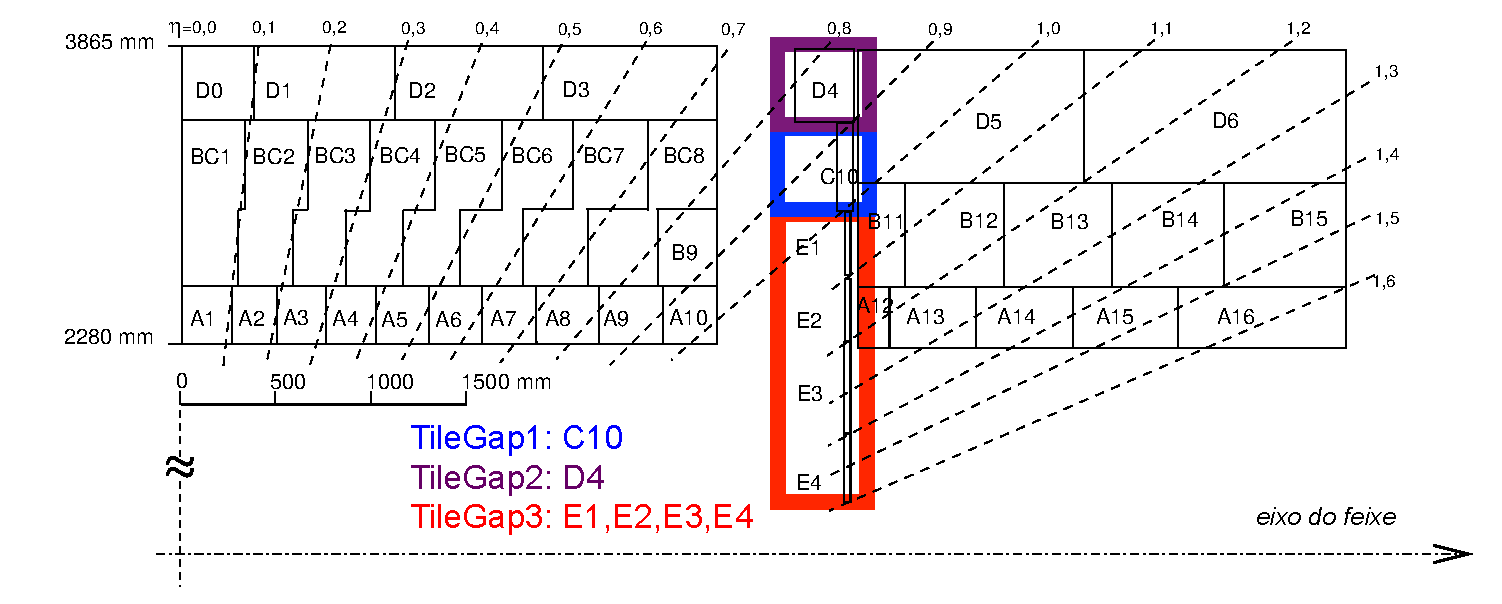
\includegraphics[width=\textwidth]{appendices/figures/tilegap.pdf}
\caption{Schematic slice of the barrel (left), extended barrel (right) and
  intermediate calorimeter (highlighted) cells of the \tilecal.}%
\label{fig:tilecal_cells}
\end{figure}

\FloatBarrier{}
\newpage
\subsection{MLP Output for Simulated and Collision Data}\label{ssec:mcdata_nnoutput}

Figure~\ref{fig:mcdata_nnoutput} shows the effect of simulation mis-modellings
in the MLP output, where a shift towards negative values (more background-like)
are seen for both signal and background data. We did not employ pile-up
reweighing tools on MC data for the generation of these plots, hence the
profiles are observed with different pile-up conditions.

\begin{figure}[ht]
  \centering
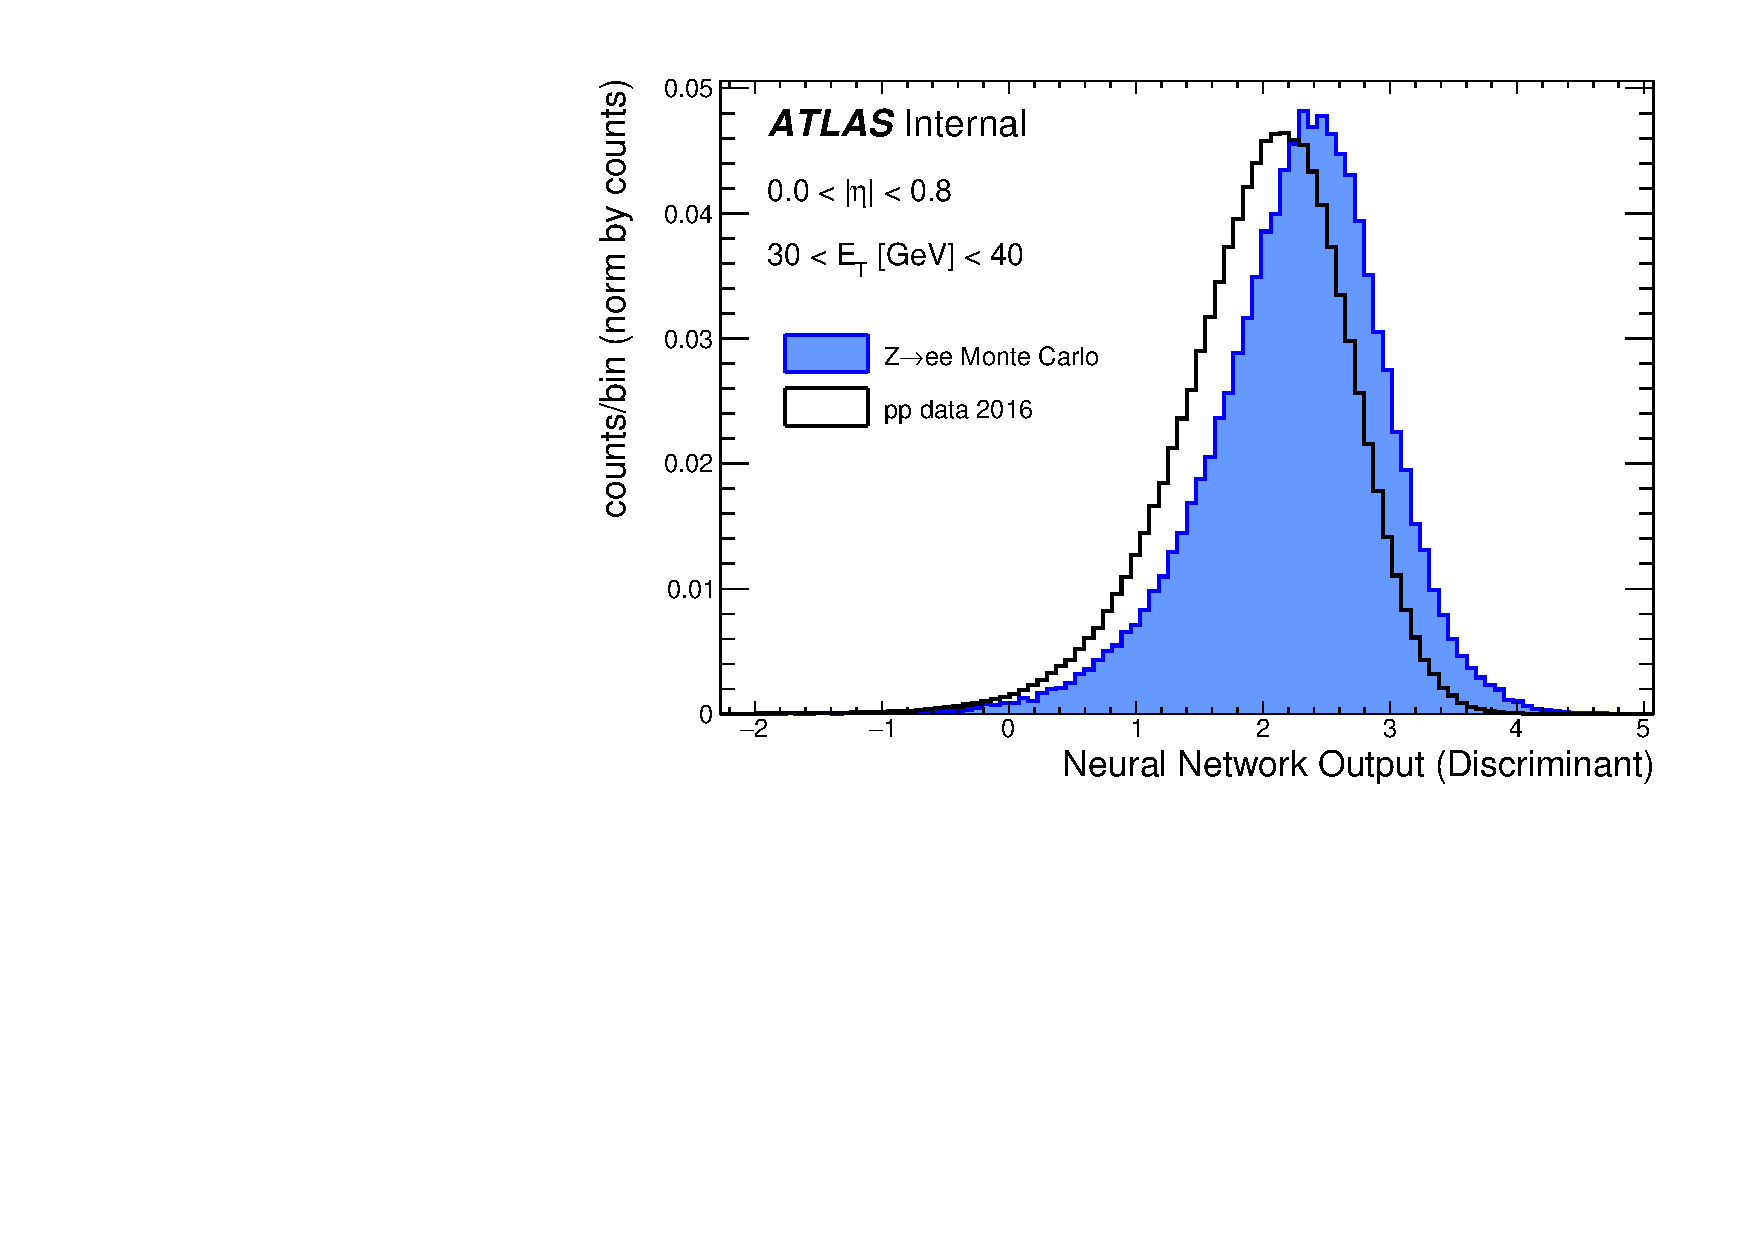
\includegraphics[width=0.8\textwidth]{appendices/figures/nn_output_mc15_versus_data16_et2_eta0.pdf}
\caption{MLP outputs for 2017 \rnn{} tunes for 
regions $30 < \et{} [\GeV] < 40$ and $0.0 < |\eta| < 0.8$ slice.\label{fig:mcdata_nnoutput}.}
\end{figure}


\subsection{MLP Topology}
\label{ssec:mlp_topo}

We should include some description here.




\begin{table}[ht!]
\scriptsize
\resizebox{1.000000\textwidth}{!}{%
\begin{tabular}
{lccccccc}
\hline
\hline
&  & $15 < E_{T} \text{[Gev]}<20$ & $20 < E_{T} \text{[Gev]}<30$ & $30 < E_{T} \text{[Gev]}<40$ & $40 < E_{T} \text{[Gev]}<50$ & $E_{T}\text{[GeV]} > 50$ \\
\hline
\multirow{3}{*}{$0.00<\eta<0.80$} & Input & 100 & 100 & 100 & 100 & 100 \\
& Hidden & \cellcolor[HTML]{9AFF99}5 & \cellcolor[HTML]{9AFF99}5 & \cellcolor[HTML]{9AFF99}5 & \cellcolor[HTML]{9AFF99}5 & \cellcolor[HTML]{9AFF99}5 \\
& Output & 1 & 1 & 1 & 1 & 1 \\
\hline
\multirow{3}{*}{$0.80<\eta<1.37$} & Input & 100 & 100 & 100 & 100 & 100 \\
& Hidden & \cellcolor[HTML]{9AFF99}5 & \cellcolor[HTML]{9AFF99}5 & \cellcolor[HTML]{9AFF99}5 & \cellcolor[HTML]{9AFF99}5 & \cellcolor[HTML]{9AFF99}5 \\
& Output & 1 & 1 & 1 & 1 & 1 \\
\hline
\multirow{3}{*}{$1.37<\eta<1.54$} & Input & 100 & 100 & 100 & 100 & 100 \\
& Hidden & \cellcolor[HTML]{9AFF99}7 & \cellcolor[HTML]{9AFF99}19 & \cellcolor[HTML]{9AFF99}13 & \cellcolor[HTML]{9AFF99}13 & \cellcolor[HTML]{9AFF99}6 \\
& Output & 1 & 1 & 1 & 1 & 1 \\
\hline
\multirow{3}{*}{$1.54<\eta<2.50$} & Input & 100 & 100 & 100 & 100 & 100 \\
& Hidden & \cellcolor[HTML]{9AFF99}5 & \cellcolor[HTML]{9AFF99}15 & \cellcolor[HTML]{9AFF99}5 & \cellcolor[HTML]{9AFF99}5 & \cellcolor[HTML]{9AFF99}5 \\
& Output & 1 & 1 & 1 & 1 & 1 \\
\hline
\hline
\end{tabular}
}
\caption{Number of neuron in hidden layer for 2017 operation.}
\label{tab:neurons_v6}
\end{table}


\begin{table}[ht!]
    \scriptsize
    \resizebox{1.000000\textwidth}{!}{%
    \begin{tabular}
    {lccccccc}
    \hline
    \hline
    &  & $15 < E_{T} \text{[Gev]}<20$ & $20 < E_{T} \text{[Gev]}<30$ & $30 < E_{T} \text{[Gev]}<40$ & $40 < E_{T} \text{[Gev]}<50$ & $E_{T}\text{[GeV]} > 50$ \\
    \hline
    \multirow{3}{*}{$0.00<\eta<0.80$} & Input & 100 & 100 & 100 & 100 & 100 \\
    & Hidden & \cellcolor[HTML]{9AFF99}5 & \cellcolor[HTML]{9AFF99}5 & \cellcolor[HTML]{9AFF99}5 & \cellcolor[HTML]{9AFF99}5 & \cellcolor[HTML]{9AFF99}5 \\
    & Output & 1 & 1 & 1 & 1 & 1 \\
    \hline
    \multirow{3}{*}{$0.80<\eta<1.37$} & Input & 100 & 100 & 100 & 100 & 100 \\
    & Hidden & \cellcolor[HTML]{9AFF99}5 & \cellcolor[HTML]{9AFF99}5 & \cellcolor[HTML]{9AFF99}5 & \cellcolor[HTML]{9AFF99}5 & \cellcolor[HTML]{9AFF99}5 \\
    & Output & 1 & 1 & 1 & 1 & 1 \\
    \hline
    \multirow{3}{*}{$1.37<\eta<1.54$} & Input & 100 & 100 & 100 & 100 & 100 \\
    & Hidden & \cellcolor[HTML]{9AFF99}5 & \cellcolor[HTML]{9AFF99}5 & \cellcolor[HTML]{9AFF99}5 & \cellcolor[HTML]{9AFF99}5 & \cellcolor[HTML]{9AFF99}5 \\
    & Output & 1 & 1 & 1 & 1 & 1 \\
    \hline
    \multirow{3}{*}{$1.54<\eta<2.37$} & Input & 100 & 100 & 100 & 100 & 100 \\
    & Hidden & \cellcolor[HTML]{9AFF99}5 & \cellcolor[HTML]{9AFF99}5 & \cellcolor[HTML]{9AFF99}5 & \cellcolor[HTML]{9AFF99}5 & \cellcolor[HTML]{9AFF99}5 \\
    & Output & 1 & 1 & 1 & 1 & 1 \\
    \hline
    \multirow{3}{*}{$2.37<\eta<2.50$} & Input & 100 & 100 & 100 & 100 & 100 \\
    & Hidden & \cellcolor[HTML]{9AFF99}5 & \cellcolor[HTML]{9AFF99}5 & \cellcolor[HTML]{9AFF99}5 & \cellcolor[HTML]{9AFF99}5 & \cellcolor[HTML]{9AFF99}5 \\
    & Output & 1 & 1 & 1 & 1 & 1 \\
    \hline
    \hline
    \end{tabular}
    }
    \caption{Number of neuron in hidden layer for 2018 operation.}
    \label{tab:neurons_v8}
    \end{table}
    



\subsection{Monitoring Histograms of \fastcalo Algorithms Total CPU
Time}\label{ssec:fastcalo_monitoring}

During Run~2, \fastcalo feature extraction algorithm executed sequentially the
following tools: ESamp2 (EM2 shower shapes), ESamp1 (EM1 shower shapes), EaEm
(raw EM energy) and EHadEn (raw HAD energy). The CPU time obtained using the
monitoring tool for the electron trigger without \rnn are available in
Figure~\ref{fig:fastcalo_fex_tools_time}.

\begin{figure}[ht]
\begin{subfigure}[c]{.48\textwidth}
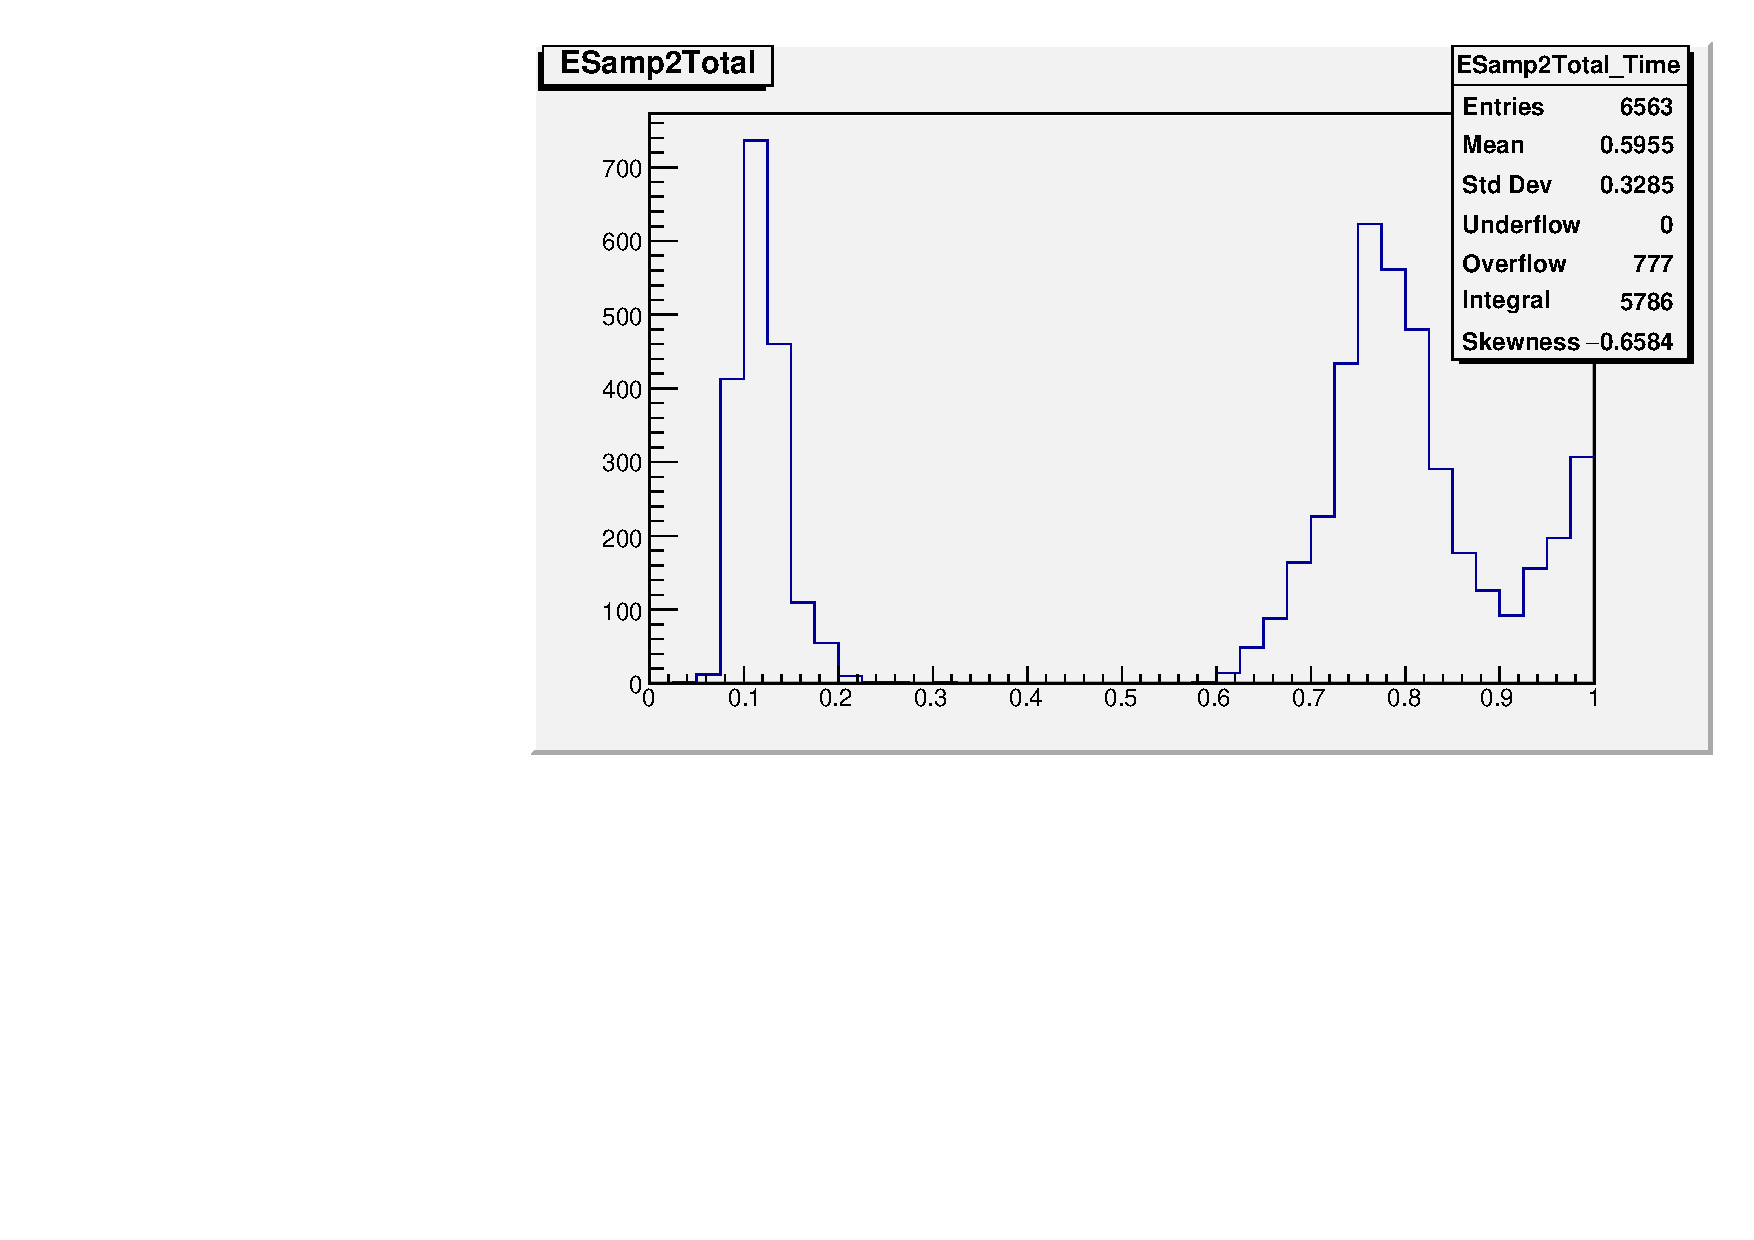
\includegraphics[width=\textwidth]{appendices/figures/fastcalo_time/samp2.pdf}
\centering
\end{subfigure}
\begin{subfigure}[c]{.48\textwidth}
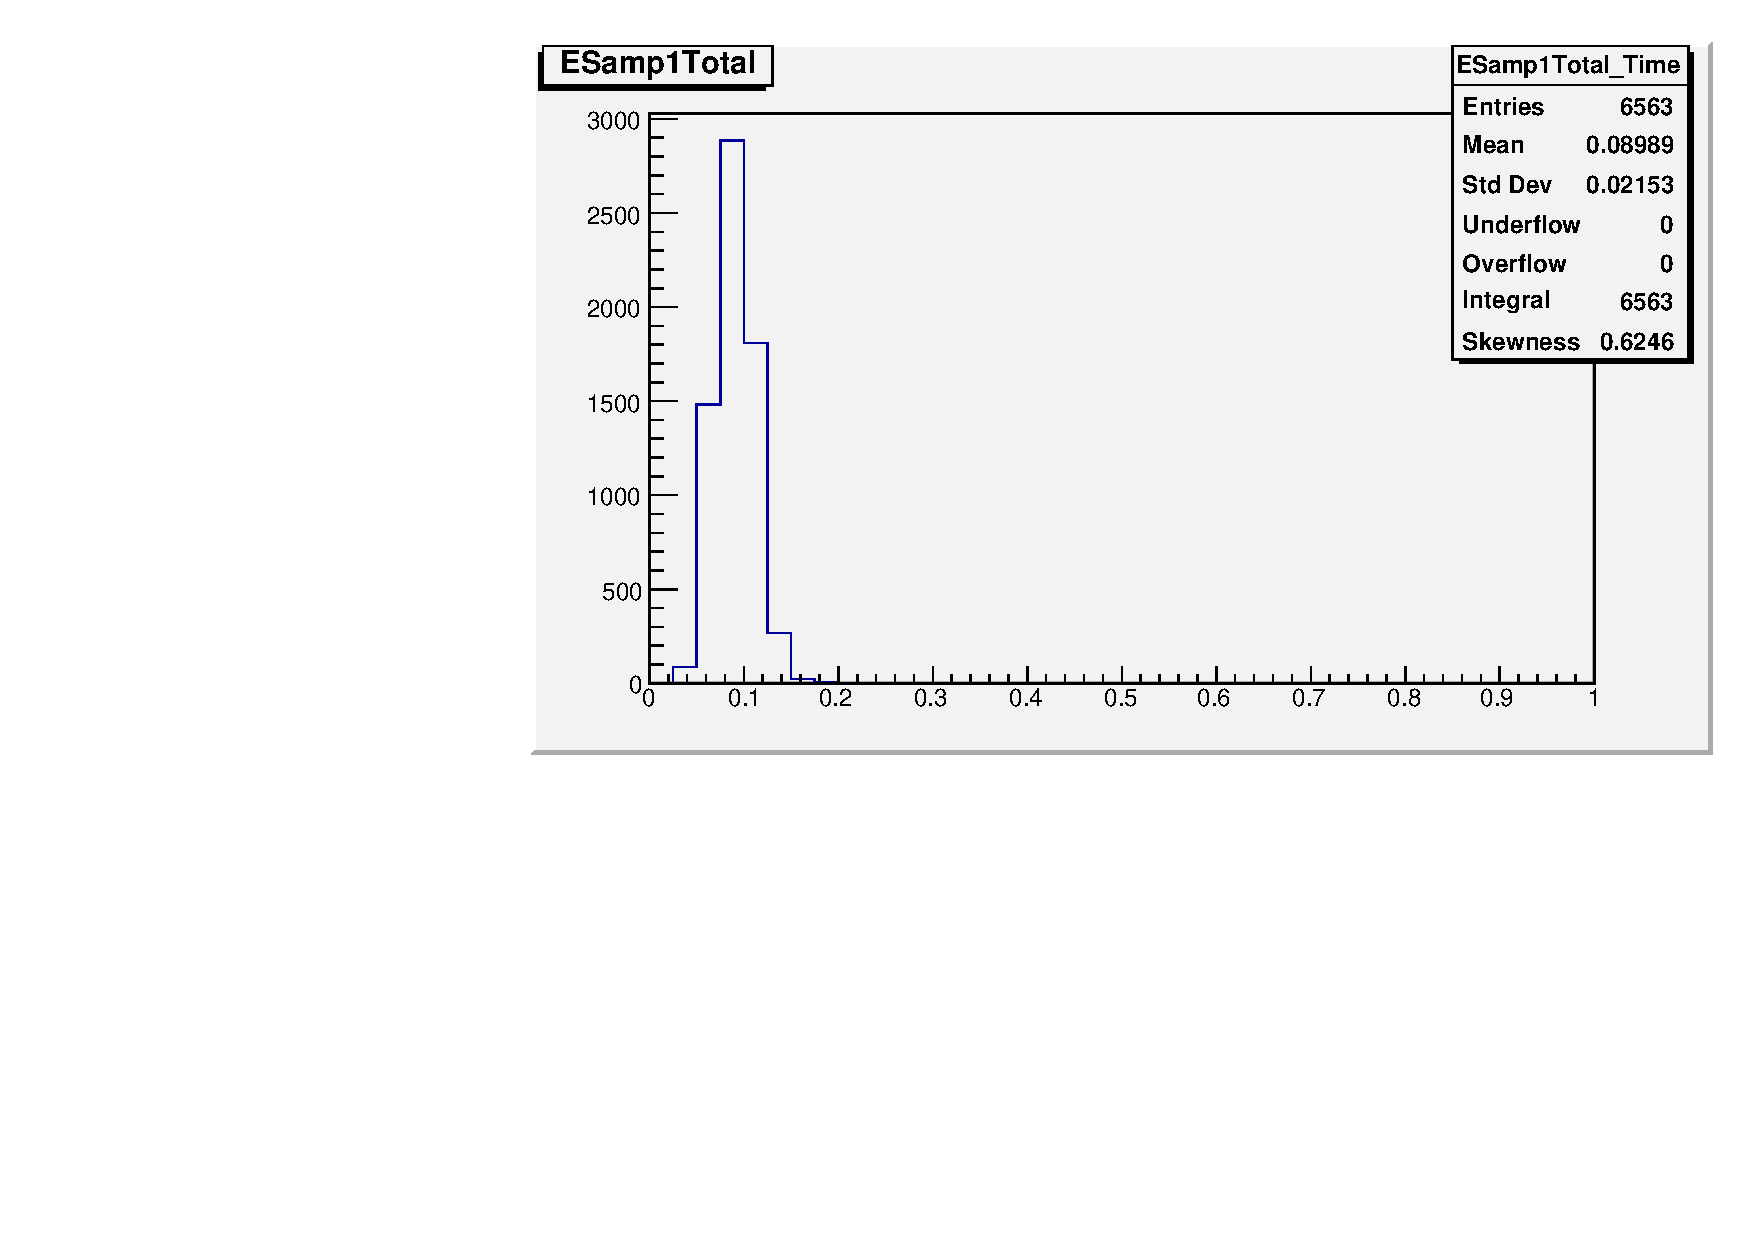
\includegraphics[width=\textwidth]{appendices/figures/fastcalo_time/samp1.pdf}
\centering
\end{subfigure} \\
\begin{subfigure}[c]{.48\textwidth}
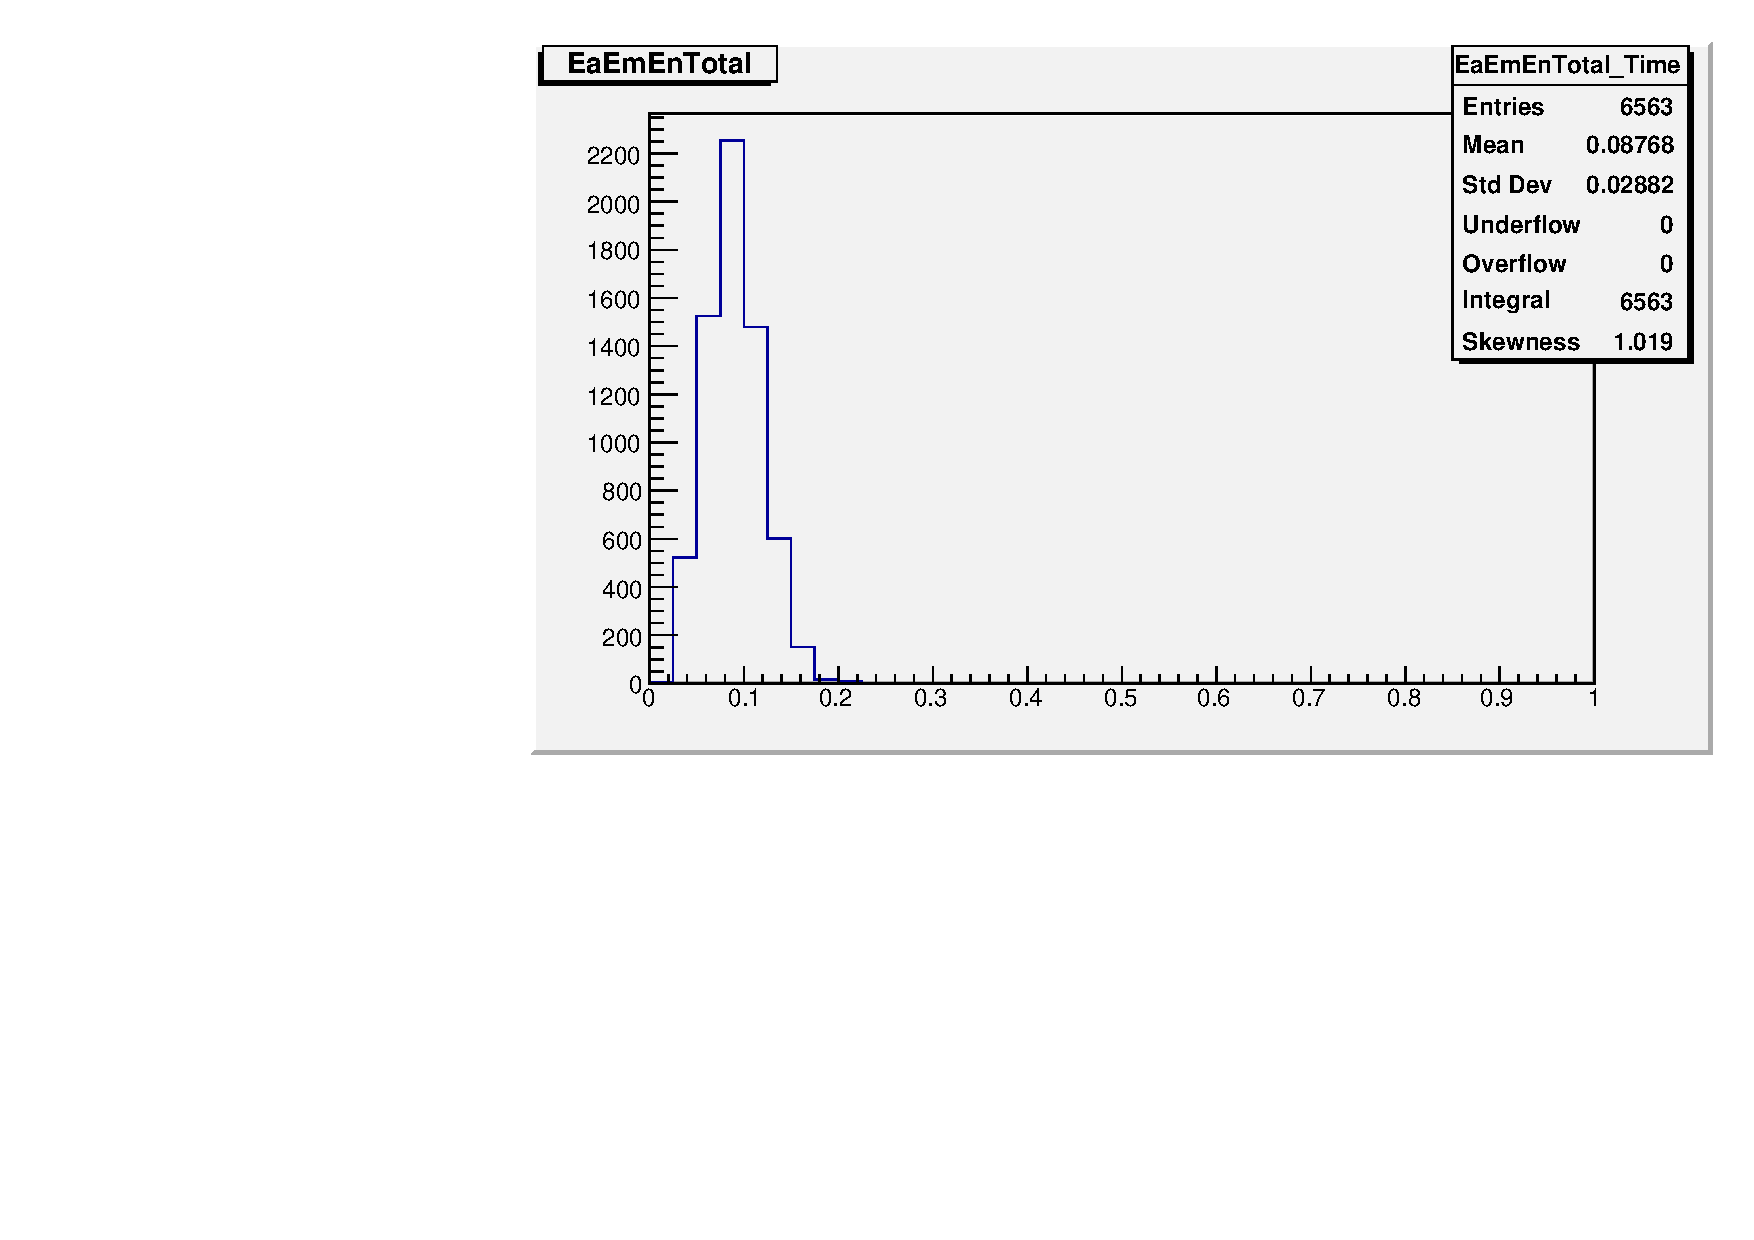
\includegraphics[width=\textwidth]{appendices/figures/fastcalo_time/ementotal.pdf}
\centering
\end{subfigure}
\begin{subfigure}[c]{.48\textwidth}
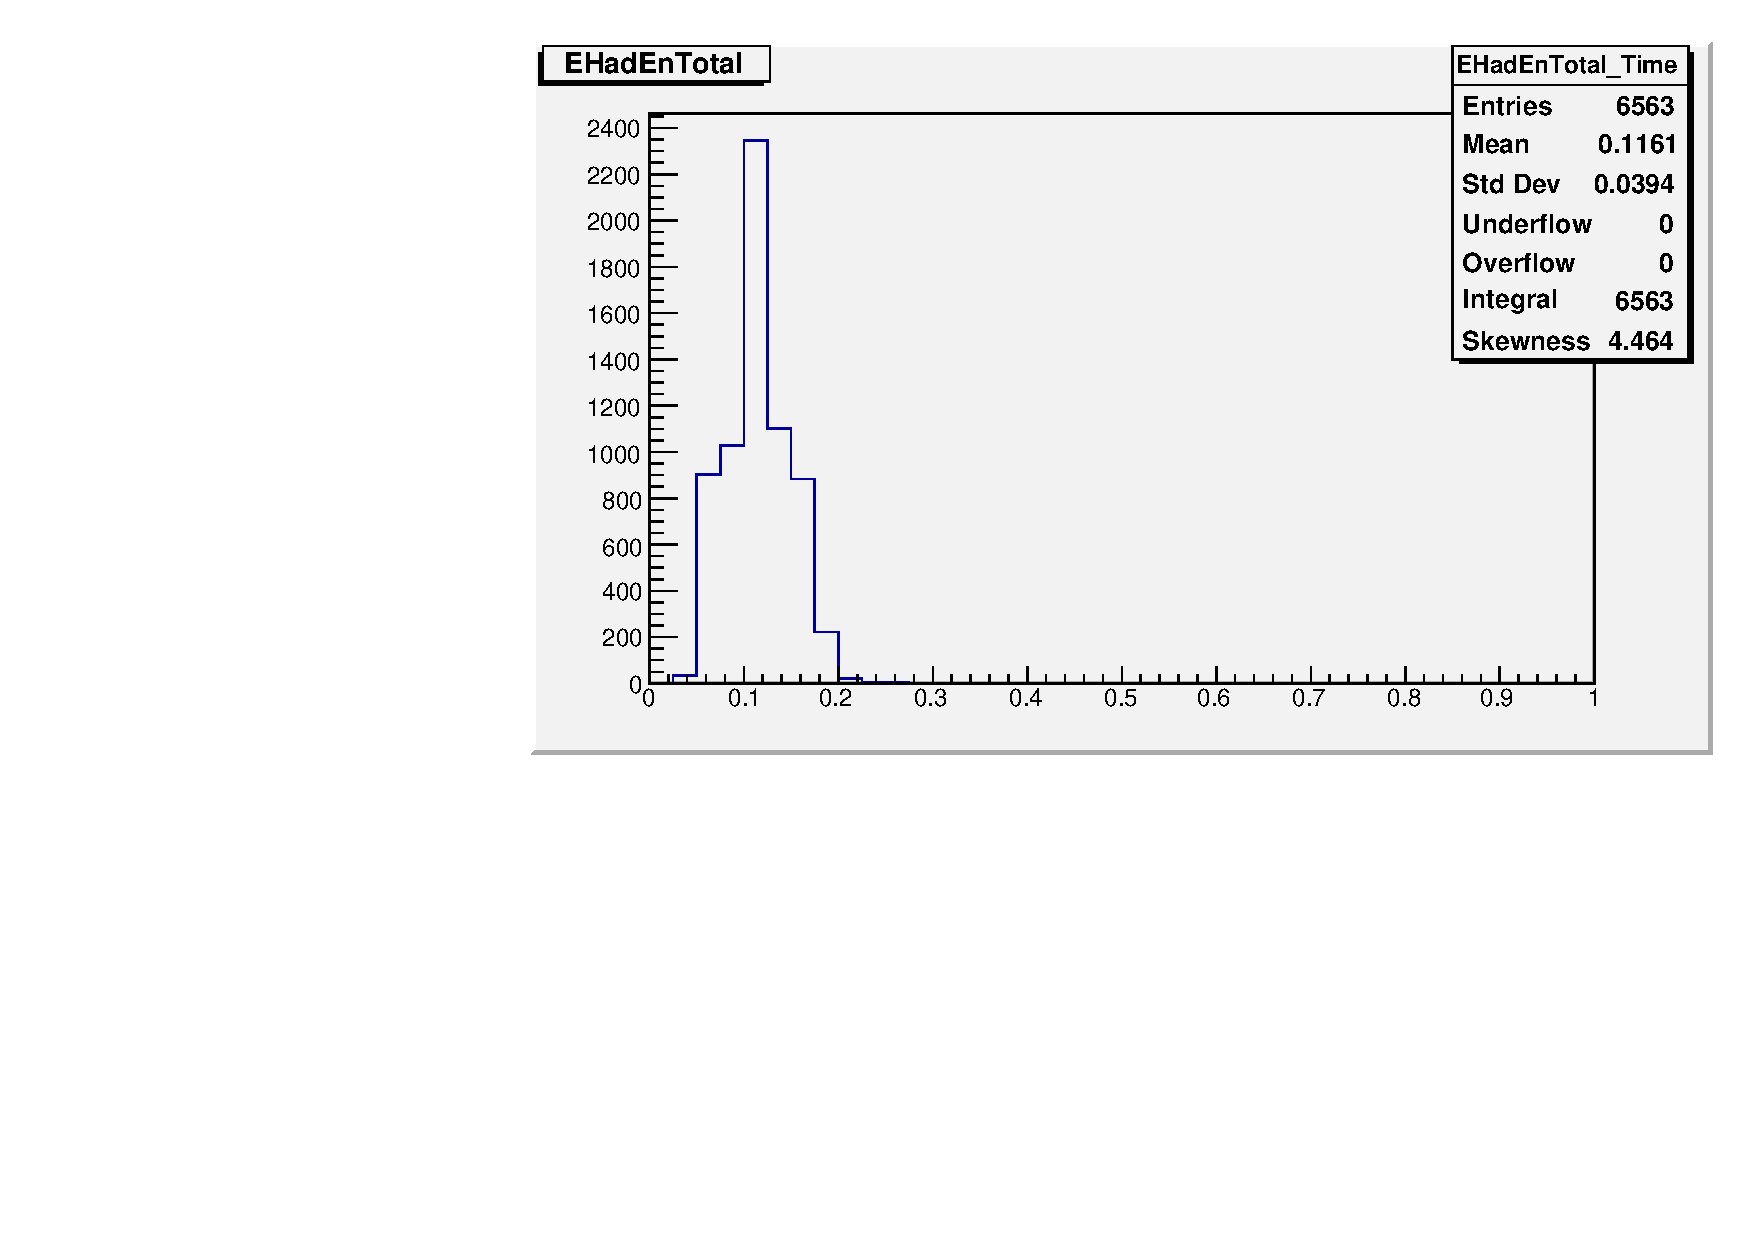
\includegraphics[width=\textwidth]{appendices/figures/fastcalo_time/ehadtotal.pdf}
\centering
\end{subfigure}
\caption{CPU time in the monitoring tool for each \fastcalo tool (except for
calibration). The histograms are shown for the electron trigger without \rnn.
Measurement configuration is described in Figure~\ref{fig:fastcalo_fex_time}.}%
\label{fig:fastcalo_fex_tools_time}
\end{figure}

\subsection{Multi-modal CPU time structure of ESamp2 Algorithm}\label{ssec:esamp2}

The multi-modal distribution observed in ESamp2 total CPU time
(Figure~\ref{fig:fastcalo_fex_tools_time}) is mainly
(Figure~\ref{fig:fastcalo_samp2_contributions}) due to the retrieval of
the EM2 cells information (ESamp2BSCnv), but also observed in ESamp2Reg with
lower central values. The two peaks around \SI{0.7}{\ms/\text{event}} and
\SI{0.9}{\ms/\text{event}} are one of the largest contributions to the total
\fastcalo CPU time.

\begin{figure}[ht]
\begin{subfigure}[c]{.48\textwidth}
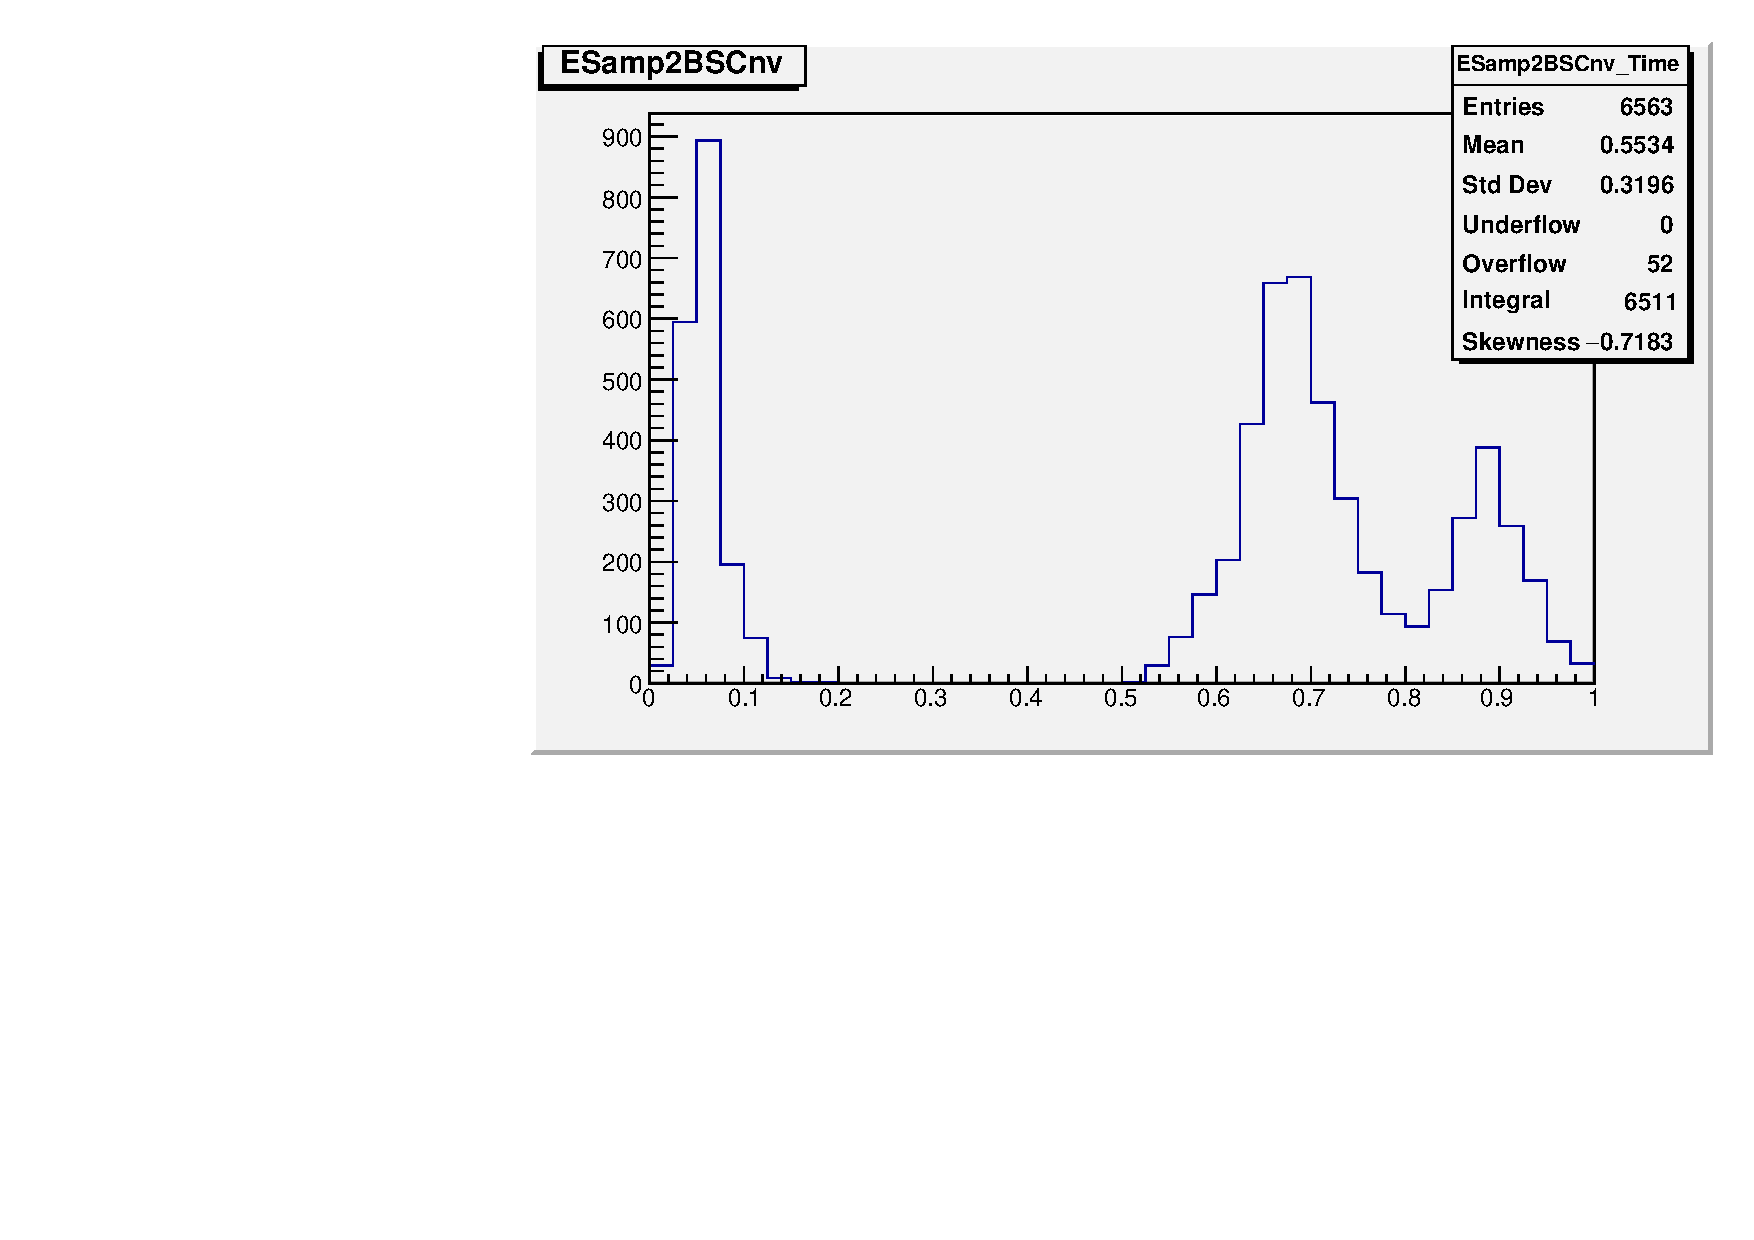
\includegraphics[width=\textwidth]{appendices/figures/fastcalo_time/ESamp2BSCnv.pdf}
\centering
\end{subfigure}
\begin{subfigure}[c]{.48\textwidth}
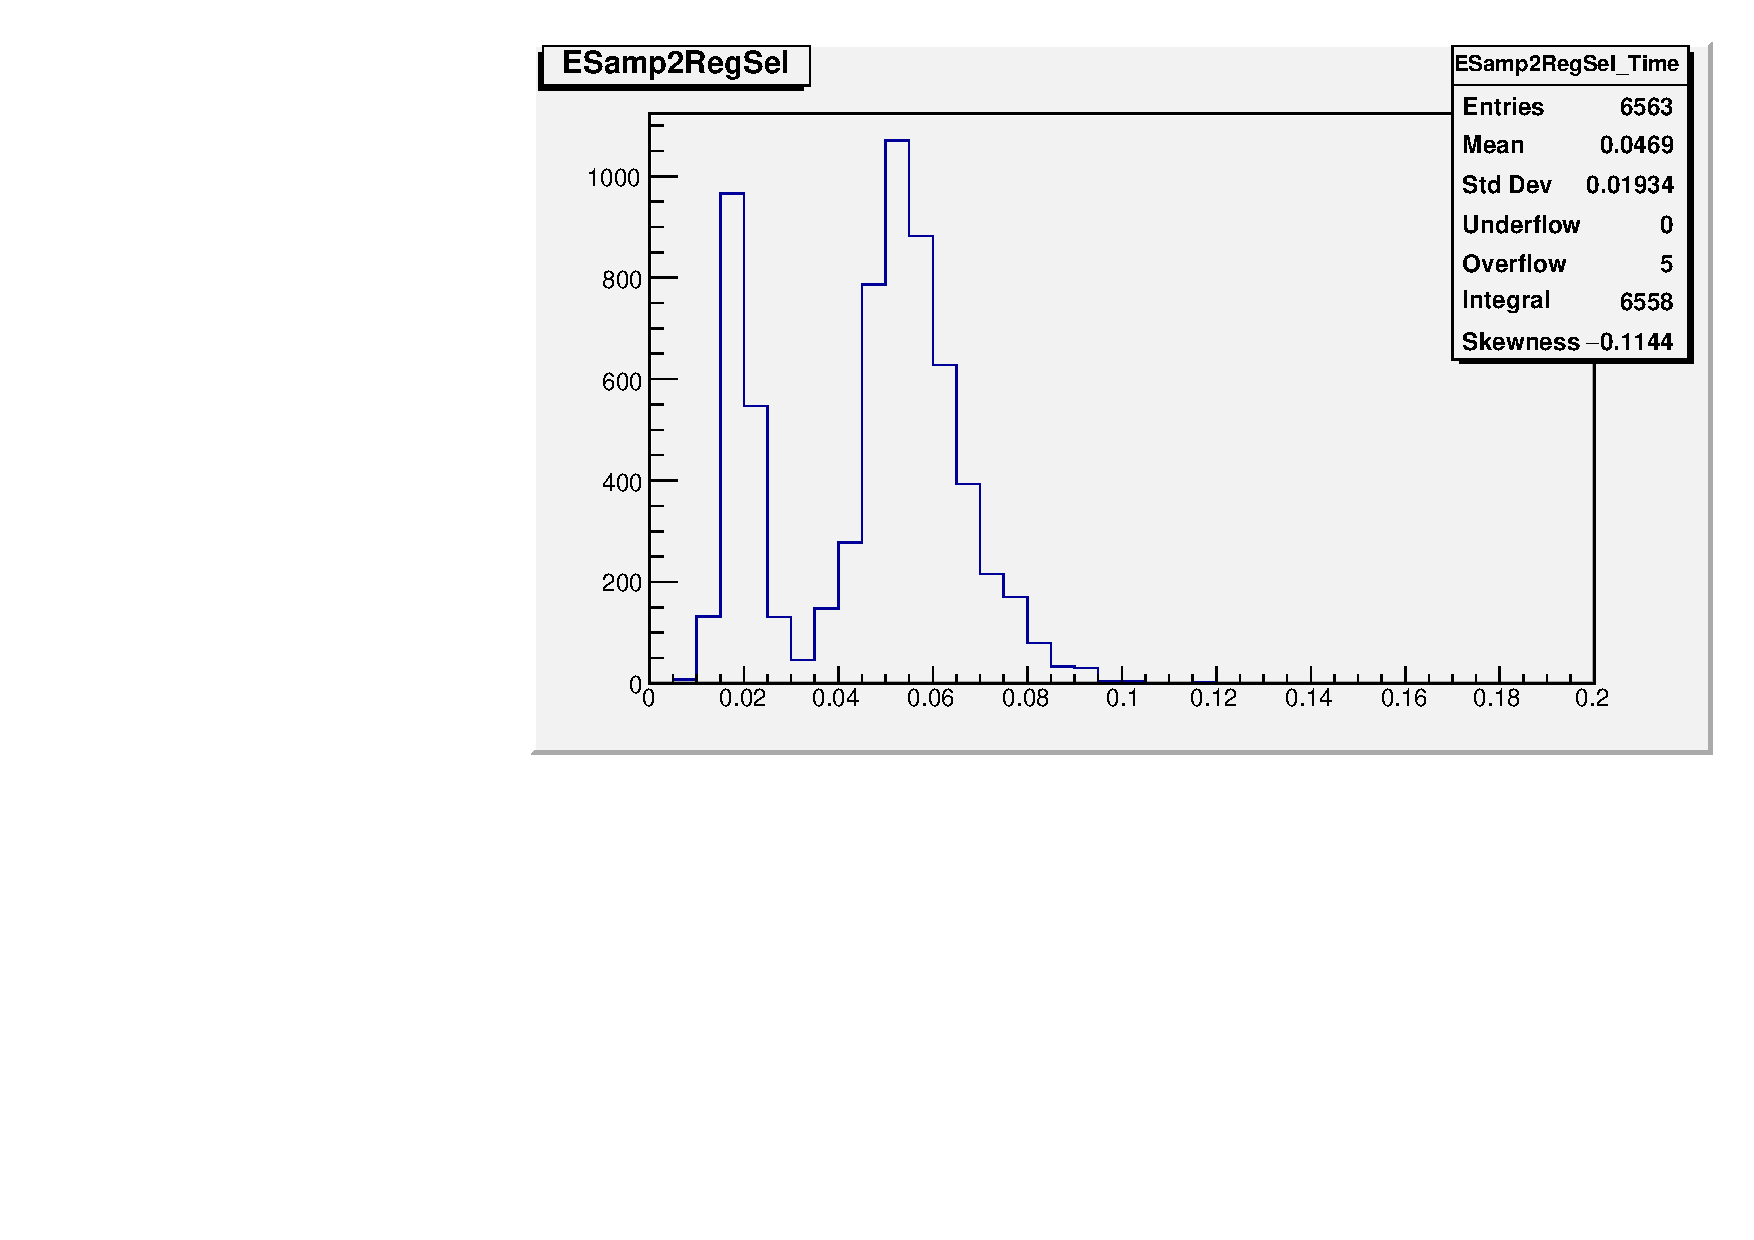
\includegraphics[width=\textwidth]{appendices/figures/fastcalo_time/ESamp2Reg.pdf}
\centering
\end{subfigure} \\
\centering
\caption{CPU time of particular computations in the ESamp2 algorithm. The
histograms are shown for the electron trigger without \rnn.  Measurement
configuration is described in Figure~\ref{fig:fastcalo_fex_time}.}%
\label{fig:fastcalo_samp2_contributions}
\end{figure}

\FloatBarrier

%\subsection{Lowest-Threshold Unprescaled Isolated Single-Electron Trigger Rate
%with respect to Luminosity}\label{ssec:primary_rate_wrt_luminosity}
%
%Figure~\ref{fig:primary_trigger_rate_wrt_lumi} shows similar trigger rates with
%respect to instantaneous luminosity for the period 2015--2018.
%
%\begin{figure}[t]
%  \centering
%  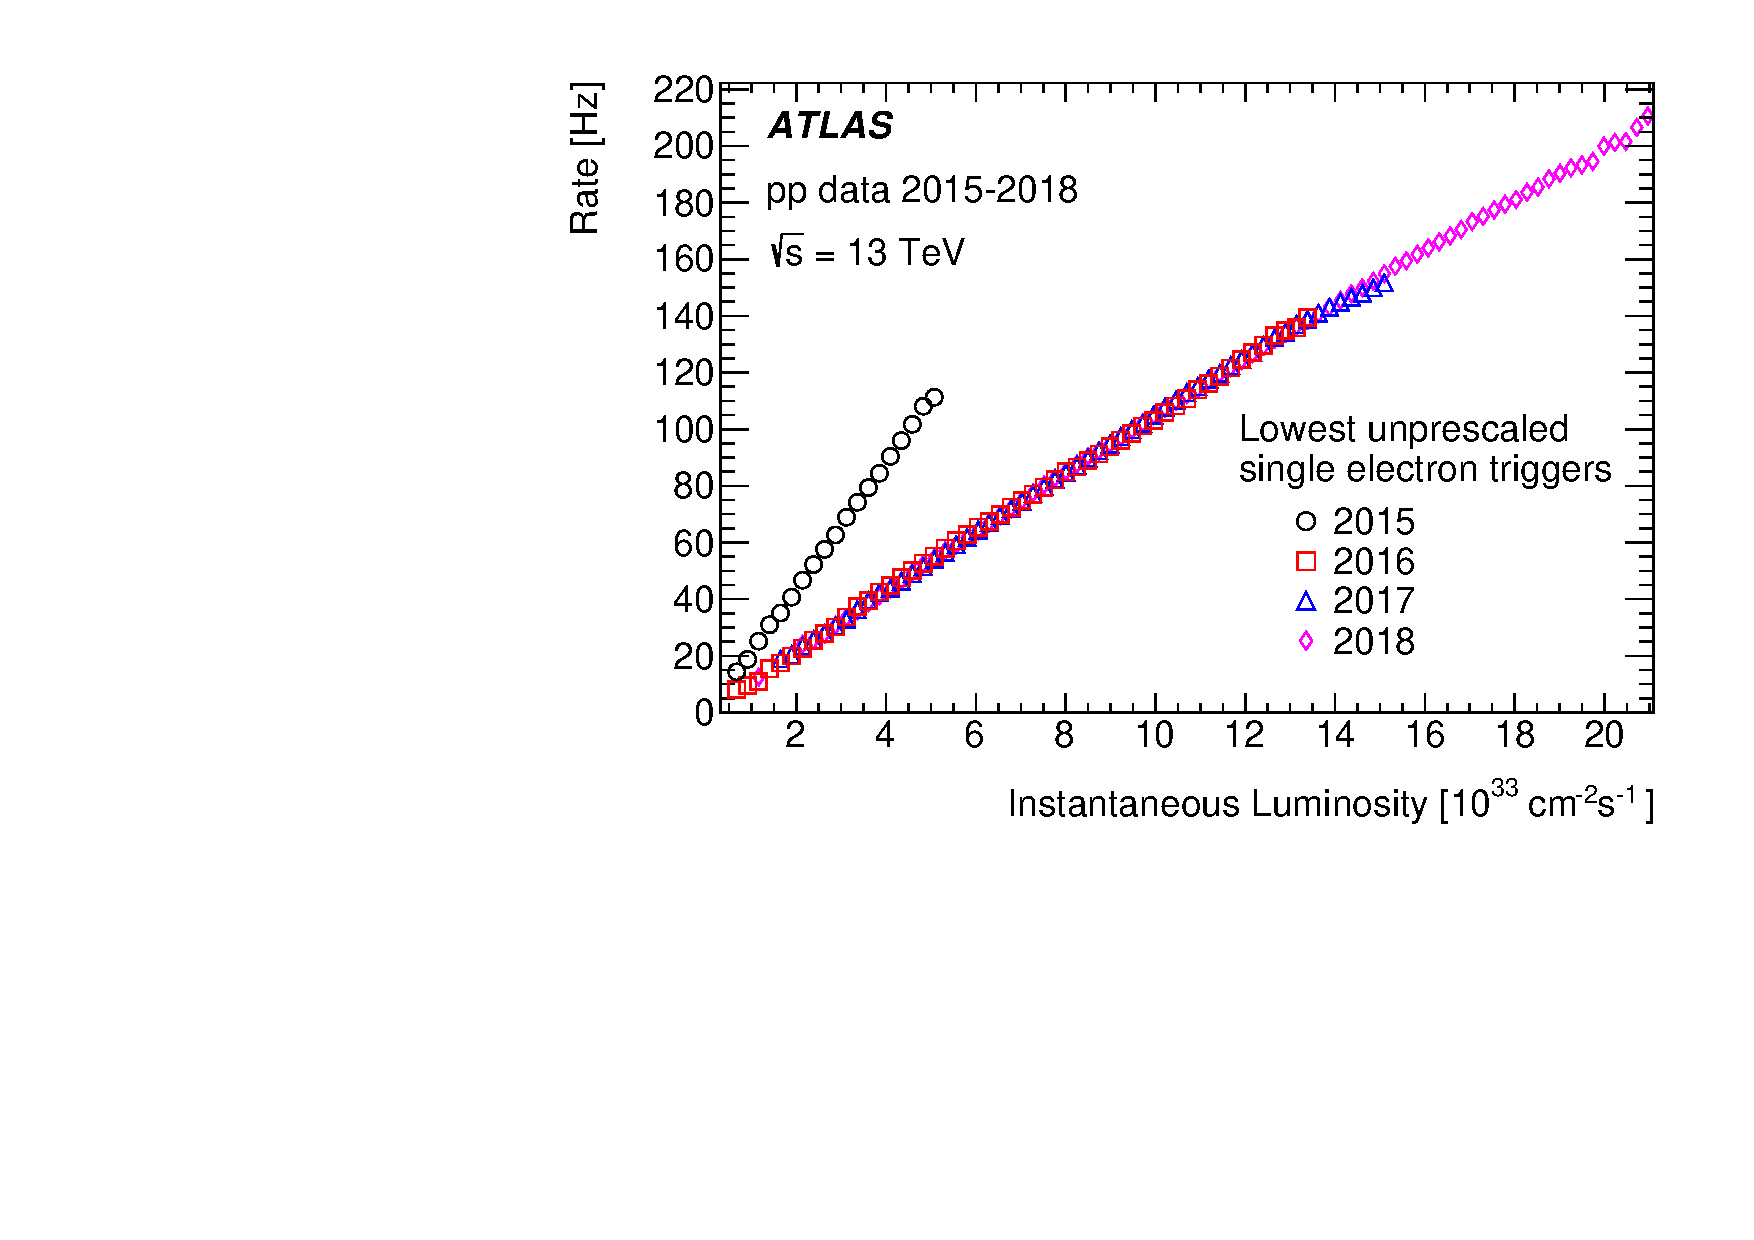
\includegraphics[width=.6\textwidth]{public_plots/fig_14}
%  \caption{\label{fig:primary_trigger_rate_wrt_lumi}Dependence of the trigger
%  rate on the luminosity for the lowest-threshold unprescaled isolated
%single-electron triggers in 2015--2018.}
%\end{figure}
%
\subsection{Background Efficiency Measurement for 2017
Cost Monitoring}\label{ssec:2017_cost_background_eff}

Estimations using the cost monitoring duplicated triggers in different
runs are shown in Table~\ref{tab:results_commissioning_v6_cost_monitoring}.
\rnn improvements range from 1.5 to 5$\times$\footnote{Specifically
for the configuration and trigger evaluated on
Figure~\ref{fig:fastcalo_fex_time}, a 1.5$\times$ reduction factor is obtained.}
and are dependent on both the trigger \et and selection requirements.

\begin{table}[ht!]
    \centering
    \caption{\label{tab:results_commissioning_v6_cost_monitoring}%
    Total number of \fastcalo and \fastelectron executions requested per monitored
    trigger in CPU cost evaluations ATR-16656 (run 309640) and ATR-16657 (run
    327265) using the final 2017 \rnn configuration and evaluated in the nightly release
    AtlasP1-21.1-2017-07-01. The reduction factor is computed as the fraction of
    \fastelectron executions in previous trigger (without \rnn) with respect to
    proposed trigger (with \rnn). See~\cite{Pinto2017} for more details.
    }
    \resizebox{\textwidth}{!}{%
    \begin{tabular}{%
    llr
    S[table-format=4.0, table-number-alignment=center,
    round-mode=figures, round-precision=2]
    c
    }
    \hline \hline
    run &
    \multirow{2}{*}{trigger} &
    %\begin{tabular}[c]{@{}c@{}}\fastcalo \\
    %(calls)\end{tabular}
    \multicolumn{1}{c}{\fastcalo} &
    \multicolumn{1}{c}{\fastelectron} &
    \multicolumn{1}{c}{Reduction} \\ \cline{3-4}
    \multicolumn{1}{c}{number} &
    &
    \multicolumn{2}{c}{Total Executions $\times 10^{-3}$ } &
    \multicolumn{1}{c}{Factor} \\
    \hline \hline
    \multirow{6}{*}{309640} & e17\_lhvloose\_nod0\_noringer\_L1EM15VHI &
    \multirow{2}{*}{\numRF{17989.136}{2}} & 8984.315 &
    \multicolumn{1}{c}{\multirow{2}{*}{1.71$\times$}} \\ \cline{4-4}
    
    & e17\_lhvloose\_nod0\_L1EM15VHI &  & 5234.167 &  \\ \cline{2-5}
    
    & e28\_lhtight\_nod0\_noringer\_ivarloose\_L1EM24VHIM &
    \multirow{2}{*}{\numRF{3084.292}{2}} & 1046.078 &
    \multicolumn{1}{c}{\multirow{2}{*}{1.69$\times$}} \\ \cline{4-4}
    
    & e28\_lhtight\_nod0\_ivarloose\_L1EM24VHIM &  & 618.011 &  \\ \cline{2-5}
    
    & e60\_lhmedium\_nod0\_noringer\_L1EM24VHIM & \multirow{2}{*}{\numRF{3084.292}{2}} &
    1046.078 & \multicolumn{1}{c}{\multirow{2}{*}{4.91$\times$}} \\ \cline{4-4}
    
    & e60\_lhmedium\_nod0\_L1EM24VHIM &  & 213.037 &  \\ \hline \hline
    
    \multicolumn{1}{l}{\multirow{6}{*}{327265}} &
    e17\_lhvloose\_nod0\_noringer\_L1EM15VHI & \multirow{2}{*}{\numRF{15609.134}{2}}
    & 7400.864 &
    \multicolumn{1}{c}{\multirow{2}{*}{1.52$\times$}} \\ \cline{4-4}
    
    \multicolumn{1}{l}{} & e17\_lhvloose\_nod0\_L1EM15VHI &  & 4855.326 &
    \multicolumn{1}{l}{} \\ \cline{2-5}
    
    \multicolumn{1}{l}{} & e28\_lhtight\_nod0\_noringer\_ivarloose\_L1EM24VHIM &
    \multirow{2}{*}{\numRF{3296.808}{2}} & 1150.932 &
    \multicolumn{1}{c}{\multirow{2}{*}{1.58$\times$}} \\ \cline{4-4}
    
    \multicolumn{1}{l}{} & e28\_lhtight\_nod0\_ivarloose\_L1EM24VHIM &  & 725.655 &
    \multicolumn{1}{l}{} \\ \cline{2-5}
    
    \multicolumn{1}{l}{} & e60\_lhmedium\_nod0\_noringer\_L1EM24VHIM &
    \multirow{2}{*}{\numRF{3296.808}{2}} & 238.054 &
    \multicolumn{1}{c}{\multirow{2}{*}{3.10$\times$}} \\ \cline{4-4}
    
    \multicolumn{1}{l}{} & e60\_lhmedium\_nod0\_L1EM24VHIM &  & 76.735 &
    \multicolumn{1}{l}{} \\ \hline \hline
    \end{tabular}%
    }
    \end{table}



\FloatBarrier
\subsection{2016 Emulated Results}%

Table~\ref{tab:results_commissioning_v6_emulation} shows emulated results during
development stage for both collision and simulation datasets.

\begin{table}[ht]
    \begin{center}
    %\captionof{table}{%
    \caption{%
    \label{tab:results_commissioning_v6_emulation} Emulated efficiency measurements
    of the trigger e26\_lhtight\_nod0 executed with and without \rnn using 2016 menu
    version. The denominator is common for all selection stages and is the number of
    RoIs matched to an electron object reconstructed by the offline. For
    uncertainties smaller than 0.01, only central values are shown. Simulated
    dataset employed Zee and JF17 mc15 datasets (AMI tag:
    \text{e3848\_s2876\_r7917\_r7676}) respectively for signal and background
    samples. Collision data are obtained from PhysicsMain and EnhancedBias streams
    using the selection criteria in Section~\ref{ssec:dataset}.}%
    \begin{tabular}{lcccc}
    \hline
    \hline
    \hline
    Chain & FastCalo [\%] & FastElectron [\%] & HLTCalo [\%] & HLT [\%] \\
    \hline \hline
    \multicolumn{5}{c}{Run 311244} \\
    \hline
    \hline
    \multicolumn{5}{c}{Signal Efficiency} \\
    \hline \hline
    Without \rnn & $96.77 \pm 0.03$ & $96.70 \pm 0.03$ & $95.84 \pm 0.05$ & $89.74 \pm 0.07 $ \\
    \hline
    With \rnn & $96.23 \pm 0.03$ & $96.16 \pm 0.03$ & $95.31 \pm 0.04$ & $89.32 \pm 0.08$ \\
    \hline
    \hline
    \multicolumn{5}{c}{Background Efficiency} \\
    \hline
    Without \rnn & $ 16.03 \pm 0.02 $ & $15.70 \pm 0.02$ & $12.90 \pm 0.02$ & $0.57$ \\
    \hline
    \hline
    With \rnn & $ 5.41 \pm 0.02$ & $5.12 \pm 0.02$ & $3.40 \pm 0.01$ & $ 0.54 $ \\
    \hline \hline
    \multicolumn{5}{c}{Simulation} \\
    \hline \hline
    \multicolumn{5}{c}{Signal Efficiency} \\
    \hline \hline
    Without \rnn & $ 96.10 \pm 0.01 $ & $ 96.09 \pm 0.01$ &
    $95.37 \pm 0.01 $ & $89.06 \pm 0.01 $ \\
    \hline
    With \rnn & $ 96.11 \pm 0.01 $ & $ 96.09 \pm 0.01$ &
    $95.38 \pm 0.01 $ & $89.12 \pm 0.01$ \\
    \hline
    \hline
    \multicolumn{5}{c}{Background Efficiency} \\
    \hline
    \hline
    Without \rnn & $8.04 \pm 0.01$ & $7.93 \pm 0.01$ & $6.54 $ &
    $0.20$ \\
    \hline
    With \rnn & $3.69 \pm 0.01$ & $3.59 \pm 0.01$ & $2.55 $ &
    $0.19$ \\
    \hline
    \hline
    \hline
    \end{tabular}
    \end{center}
    \end{table}

\FloatBarrier
\subsection{Agreement Analysis }%
\label{ssec:agreement_extra}

\subsubsection{Homogeneity Test}%
\label{top:homogeneity_extra}

Figure~\ref{fig:probe_groups} shows that using larger periods than consecutive
luminosity blocks resulted in a small difference in the total number of counts.
The absolute difference is bounded at \SI{1.5}{\%} but typically lower than
\SI{0.2}{\%}. Figures~\ref{fig:groups_homogeneity_id}
and~\ref{fig:groups_homogeneity_caloid} show the residuals for ID and calo-ID
combined variables, respectively. Tables~\ref{tab:p_values_homogeneity}
and~\ref{tab:p_values_homogeneity_track} show that the trigger configuration has
negligible impact in the homogeneity test p-values for the offline likelihood
variables.

\begin{sidewaysfigure}[ht]
  \centering
\begin{subfigure}[c]{.32\textwidth}
\centering
\includegraphics[width=\textwidth]{appendices/figures/noAdjustment/marginal_split/e28_SplitConsecutiveFiles/base_base/probe_count0_base_base.pdf}
\caption{}%
\label{fig:probe_group0_base}
\end{subfigure}
\begin{subfigure}[c]{.32\textwidth}
\centering
\includegraphics[width=\textwidth]{appendices/figures/noAdjustment/marginal_split/e28_SplitConsecutiveFiles/base_base/delta_perc_base_base.pdf}
\caption{}%
\label{fig:probe_delta_perc_base_base}
\end{subfigure}
\begin{subfigure}[c]{.32\textwidth}
\centering
\includegraphics[width=\textwidth]{appendices/figures/noAdjustment/marginal_split/e28_SplitConsecutiveFiles/base_base/probe_count1_base_base.pdf}
\caption{}%
\label{fig:probe_group1_base}
\end{subfigure} \\
\hspace*{\fill}
\begin{subfigure}[c]{.32\textwidth}
\includegraphics[width=\textwidth]{appendices/figures/noAdjustment/marginal_split/e28_SplitConsecutiveFiles/base_new/delta_perc_base_new.pdf}
\caption{}%
\label{fig:probe_delta_perc_base_new}
\end{subfigure}
\hspace*{\fill} \\
\begin{subfigure}[c]{.32\textwidth}
\centering
\includegraphics[width=\textwidth]{appendices/figures/noAdjustment/marginal_split/e28_SplitConsecutiveFiles/new_new/probe_count0_new_new.pdf}
\caption{}%
\label{fig:probe_group0_new}
\end{subfigure}
\begin{subfigure}[c]{.32\textwidth}
\centering
\includegraphics[width=\textwidth]{appendices/figures/noAdjustment/marginal_split/e28_SplitConsecutiveFiles/new_new/delta_perc_new_new.pdf}
\caption{}%
\label{fig:probe_delta_perc_new_new}
\end{subfigure}
\begin{subfigure}[c]{.32\textwidth}
\centering
\includegraphics[width=\textwidth]{appendices/figures/noAdjustment/marginal_split/e28_SplitConsecutiveFiles/new_new/probe_count1_new_new.pdf}
\caption{}%
\label{fig:probe_group1_new}
\end{subfigure} \\
\caption{\label{fig:probe_groups}Probe counts per phase space region for the
  arbitrary first (a,e) and second (c,g) groups. First (third) line concern the probes
obtained by the trigger without (with) \rnn{}. The difference percentage between
the two groups is shown in the middle column (b,d,f). In the second line (d),
the difference percentage is computed between probe counts in first group
collected by the trigger without \rnn{} and second group collected by the
trigger with \rnn{}.}
\end{sidewaysfigure}

\FloatBarrier

\begin{figure}[b]
\begin{center}
\begin{subfigure}[c]{.48\textwidth}
\centering
\includegraphics[width=\textwidth]{appendices/figures/noAdjustment/marginal_split/e28_SplitConsecutiveFiles/base_new/el_trackd0pvunbiased_et40eta0_00_sigma_base_new.pdf}
\caption{}%
\label{fig:groups_homogeneity_d0}
\end{subfigure}
\hfill
\begin{subfigure}[c]{.48\textwidth}
\centering
\includegraphics[width=\textwidth]{appendices/figures/noAdjustment/marginal_split/e28_SplitConsecutiveFiles/base_new/el_d0significance_et40eta0_00_sigma_base_new.pdf}
\caption{}%
\label{fig:groups_homogeneity_d0sig}
\end{subfigure} \\
\begin{subfigure}[c]{.48\textwidth}
\centering
\includegraphics[width=\textwidth]{appendices/figures/noAdjustment/marginal_split/e28_SplitConsecutiveFiles/base_new/el_DeltaPoverP_et40eta0_00_sigma_base_new.pdf}
\caption{}%
\label{fig:groups_homogeneity_poverp}
\end{subfigure}
\hfill
\begin{subfigure}[c]{.48\textwidth}
\centering
\includegraphics[width=\textwidth]{appendices/figures/noAdjustment/marginal_split/e28_SplitConsecutiveFiles/base_new/el_TRT_PID_et40eta0_00_sigma_base_new.pdf}
\caption{}%
\label{fig:groups_homogeneity_trt_pid}
\end{subfigure} \\
\end{center}
\caption{%
profiles for the calo-ID combined variables employed in
the offline likelihood in the $\et>\SI{40}{\GeV}$ and $0.00<\abseta{}<0.80$
region using data collected by trigger without \rnn{} in the first arbitrary
data group (blue area) and data collected by the trigger with \rnn{} in the
second arbitrary data group (black line).
}%
\label{fig:groups_homogeneity_id}
\end{figure}%

\begin{figure}[t]
\begin{center}
\begin{subfigure}[c]{.48\textwidth}
\centering
\includegraphics[width=\textwidth]{appendices/figures/noAdjustment/marginal_split/e28_SplitConsecutiveFiles/base_new/el_deltaeta1_et40eta0_00_sigma_base_new.pdf}
\caption{}%
\label{fig:groups_homogeneity_deta}
\end{subfigure}
\begin{subfigure}[c]{.48\textwidth}
\centering
\includegraphics[width=\textwidth]{appendices/figures/noAdjustment/marginal_split/e28_SplitConsecutiveFiles/base_new/el_deltaphiRescaled_et40eta0_00_sigma_base_new.pdf}
\caption{}%
\label{fig:groups_homogeneity_dphi}
\end{subfigure}
\caption{%
profiles for the calo-ID combined variables employed in
the offline likelihood in the $\et>\SI{40}{\GeV}$ and $0.00<\abseta{}<0.80$
region using data collected by trigger without \rnn{} in the first arbitrary
data group (blue area) and data collected by the trigger with \rnn{} in the
second arbitrary data group (black line).
}%
\label{fig:groups_homogeneity_caloid}
\end{center}
\end{figure}

\FloatBarrier

\begin{table}[b]
\centering
\caption{\label{tab:p_values_homogeneity}Homogeneity test p-value and cumulated
  $\chi^2/\text{ndf}$ for the calorimeter variables and $\et{}\times\eta{}$
  regions employed to derive the offline likelihood pdfs. The lines in blue,
  yellow and green correspond respectively to the results when computing the
  test between: the trigger without the \rnn{} for the two groups; trigger with
  \rnn{} for the first and without for the second group; and trigger with the
  \rnn{} for the two groups. }
\begin{subtable}{\textwidth}
\caption{\reta{}\label{tab:p_values_reta}}
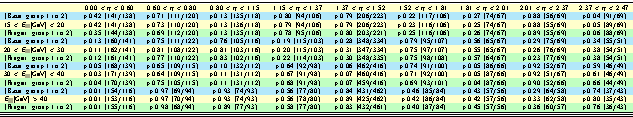
\includegraphics[width=\textwidth]{appendices/figures/homogeneity/reta_homogeneity_table.pdf}
\end{subtable} \\
\begin{subtable}{\textwidth}
\caption{\rphi{}\label{tab:p_values_rphi}}
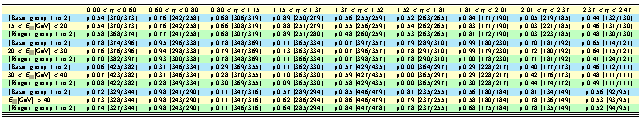
\includegraphics[width=\textwidth]{appendices/figures/homogeneity/rphi_homogeneity_table.pdf}
\end{subtable} \\
\begin{subtable}{\textwidth}
\caption{\eratio{}\label{tab:p_values_eratio}}
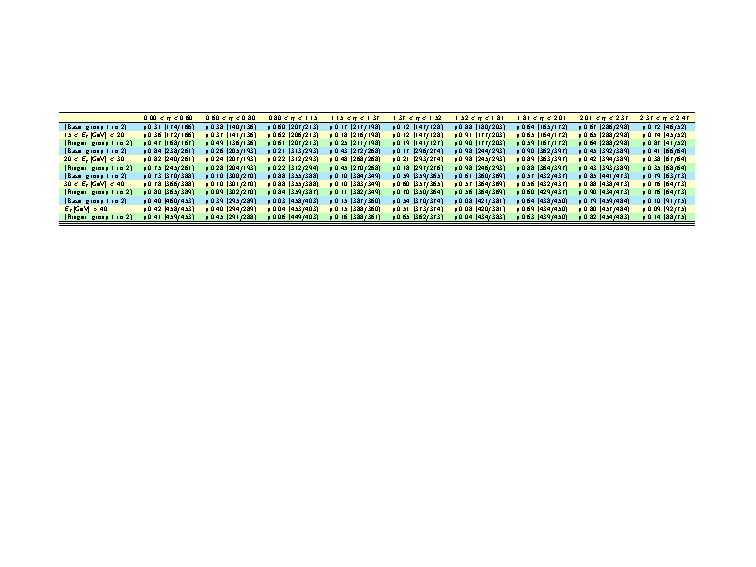
\includegraphics[width=\textwidth]{appendices/figures/homogeneity/eratio_homogeneity_table.pdf}
\end{subtable} \\
\end{table}%
\begin{table}[t]\ContinuedFloat\addtocounter{table}{-1}%
\begin{subtable}{\textwidth}
\caption{\rhad{}\label{tab:p_values_rhad}}
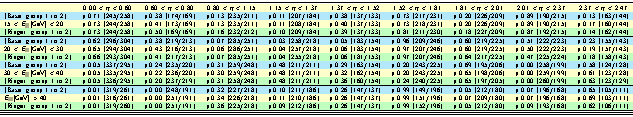
\includegraphics[width=\textwidth]{appendices/figures/homogeneity/rhad_homogeneity_table.pdf}
\end{subtable} \\
\begin{subtable}{\textwidth}
\caption{\weta{}\label{tab:p_values_weta}}
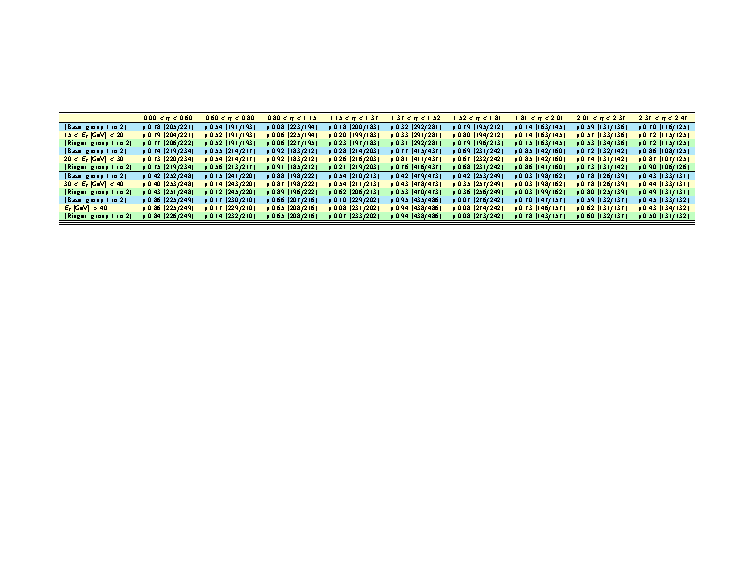
\includegraphics[width=\textwidth]{appendices/figures/homogeneity/weta2_homogeneity_table.pdf}
\end{subtable} \\
\begin{subtable}{\textwidth}
\caption{\fI{}\label{tab:p_values_f1}}
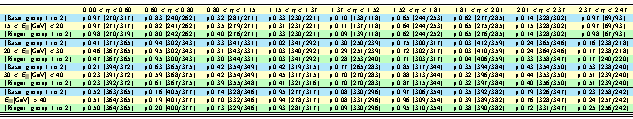
\includegraphics[width=\textwidth]{appendices/figures/homogeneity/f1_homogeneity_table.pdf}
\end{subtable} \\
\begin{subtable}{\textwidth}
\caption{\fIII{}\label{tab:p_values_f3}}
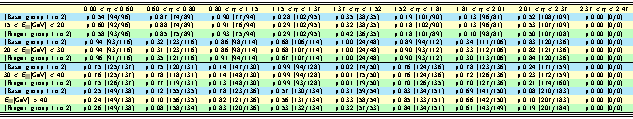
\includegraphics[width=\textwidth]{appendices/figures/homogeneity/f3_homogeneity_table.pdf}
\end{subtable} \\
\end{table}


\begin{table}[b]
\centering
\caption{\label{tab:p_values_homogeneity_track}Homogeneity test p-value and cumulated
  $\chi^2/\text{ndf}$ for the ID and calo-ID combined variables and $\et{}\times\eta{}$
  regions employed to derive the offline likelihood pdfs.}
\begin{subtable}{\textwidth}
\caption{\TRTPID{}\label{tab:p_values_trt}}
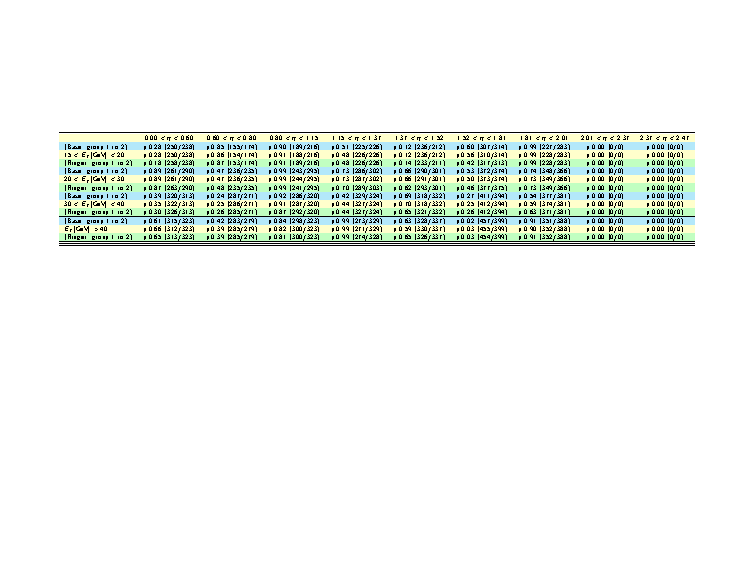
\includegraphics[width=\textwidth]{appendices/figures/homogeneity/TRT_PID_homogeneity_table.pdf}
\end{subtable} \\
\begin{subtable}{\textwidth}
\caption{\deltaeta{}\label{tab:p_values_eta}}
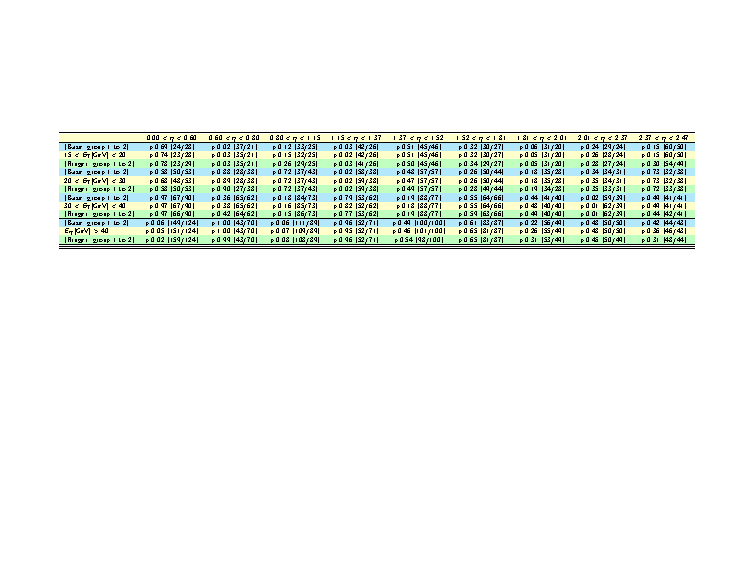
\includegraphics[width=\textwidth]{appendices/figures/homogeneity/deltaeta_homogeneity_table.pdf}
\end{subtable} \\
\begin{subtable}{\textwidth}
\caption{\deltaphires{}\label{tab:p_values_deltaphi}}
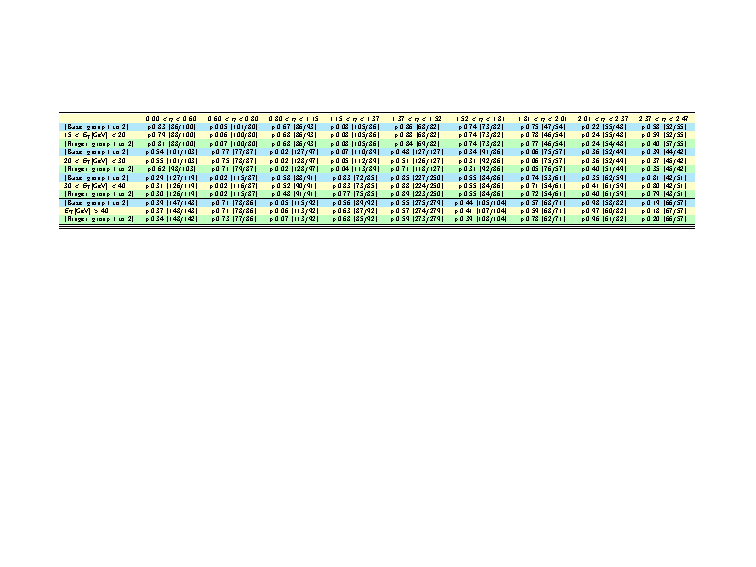
\includegraphics[width=\textwidth]{appendices/figures/homogeneity/deltaphi_homogeneity_table}
\end{subtable} \\
\end{table}
\begin{table}[t]\ContinuedFloat\addtocounter{table}{-1}
\begin{subtable}{\textwidth}
\caption{\deltapoverp{}\label{tab:p_values_poverp}}
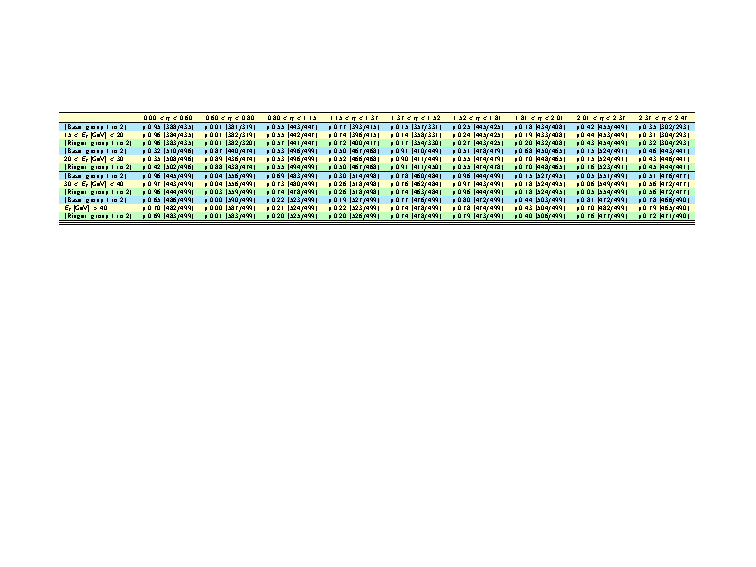
\includegraphics[width=\textwidth]{appendices/figures/homogeneity/deltapoverp_homogeneity_table.pdf}
\end{subtable} \\
\begin{subtable}{\textwidth}
\caption{\trackdO{}\label{tab:p_values_d0}}
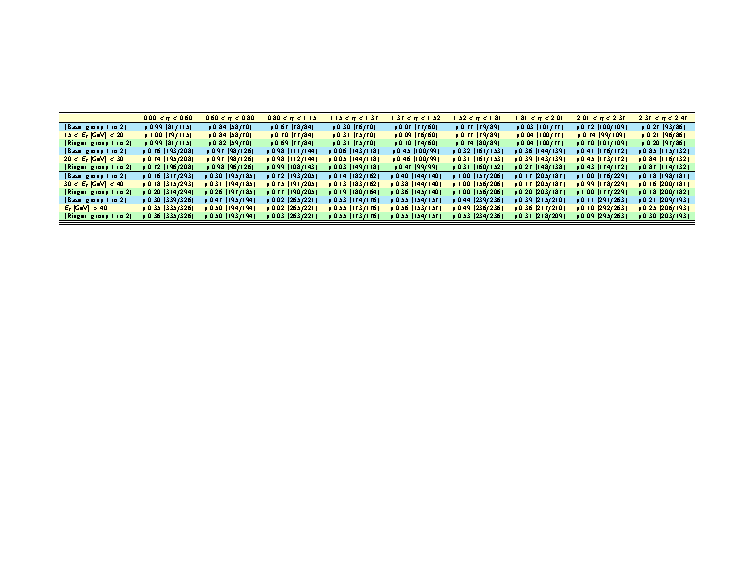
\includegraphics[width=\textwidth]{appendices/figures/homogeneity/d0_homogeneity_table.pdf}
\end{subtable} \\
\begin{subtable}{\textwidth}
\caption{\dOSignificance{}\label{tab:p_values_d0sig}}
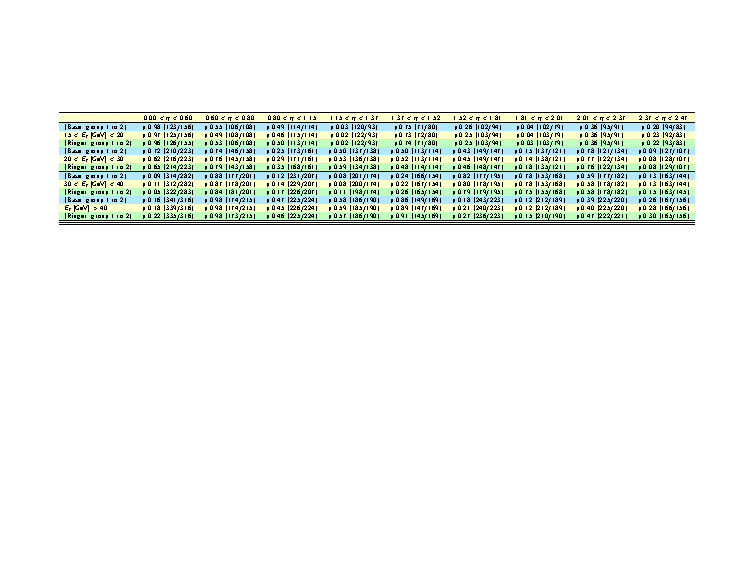
\includegraphics[width=\textwidth]{appendices/figures/homogeneity/d0significance_homogeneity_table}
\end{subtable} \\
\end{table}

\FloatBarrier
\subsubsection{Goodness-of-fit}%
\label{top:gof_extra}

Figure~\ref{fig:gof_counts} shows that the absolute difference in number of
probes is bounded around \SI{0.3}{\%}.
Table~\ref{tab:gof_chi2_p_values} and~\ref{tab:gof_ks_p_values} show the results
for $chi^2$ and KS tests, respectively. The variables relying on ID information
are shown in Figure~\ref{fig:gof_track}.

\begin{figure}[b]
\begin{center}
\begin{subfigure}[c]{.48\textwidth}
\centering
\includegraphics[width=\textwidth]{appendices/figures/noAdjustment/marginal_nosplit/e28_MergedRuns/base_new/probe_count0_base_new.pdf}
\caption{}%
\label{fig:gof_counts_without_ringer}
\end{subfigure}
\begin{subfigure}[c]{.48\textwidth}
\centering
\includegraphics[width=\textwidth]{appendices/figures/noAdjustment/marginal_nosplit/e28_MergedRuns/base_new/probe_count1_base_new.pdf}
\caption{}%
\label{fig:gof_counts_with_ringer}
\end{subfigure} \\
\hspace*{\fill}
\begin{subfigure}[c]{.48\textwidth}
\centering
\includegraphics[width=\textwidth]{appendices/figures/noAdjustment/marginal_nosplit/e28_MergedRuns/base_new/delta_perc_base_new.pdf}
\caption{}%
\label{fig:gof_delta_perc}
\end{subfigure}
\hspace*{\fill} \\
\caption{%
  Probe counts per phase space region for the trigger with (a) and without (b)
  \rnn{}. The difference percentage between the two triggers is shown at the
  bottom (c).
}%
\label{fig:gof_counts}
\end{center}
\end{figure}

\begin{table}[p]
\centering
\caption{\label{tab:gof_chi2_p_values}Goodness-of-fit $\chi^2$
KS test p-value and cumulated $\chi^2/\text{ndf}$ for all variables and
$\et{}\times\eta{}$ regions employed to derive the offline likelihood pdfs.}
\begin{subtable}{\textwidth}
\caption{\reta{}\label{tab:gof_chi2_p_values_reta}}
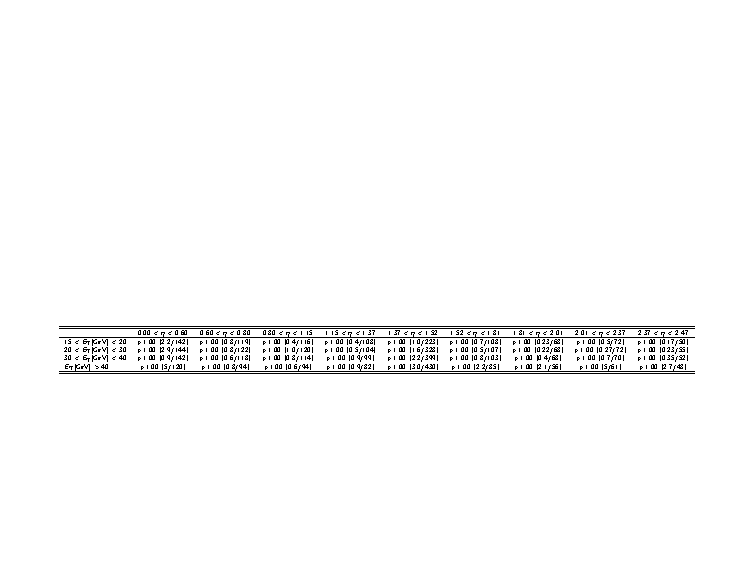
\includegraphics[width=\textwidth]{appendices/figures/gof/reta_chi2_table.pdf}
\end{subtable} \\
\begin{subtable}{\textwidth}
\caption{\rphi{}\label{tab:gof_chi2_p_values_rphi}}
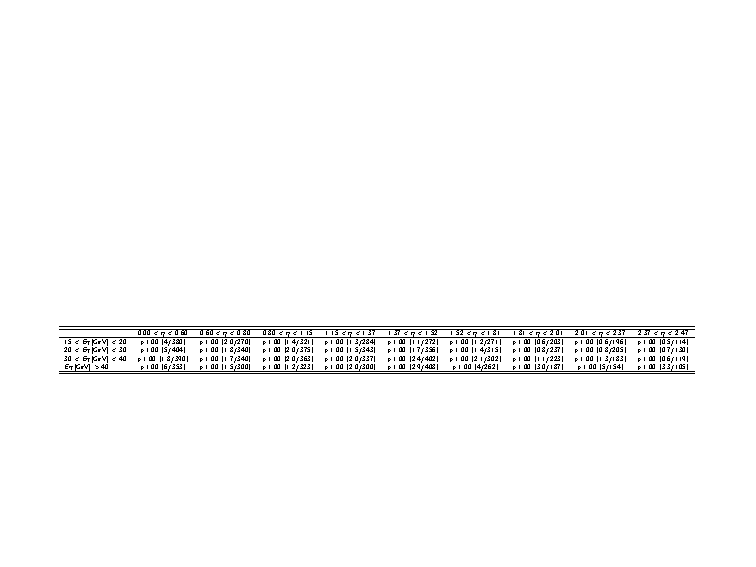
\includegraphics[width=\textwidth]{appendices/figures/gof/rphi_chi2_table.pdf}
\end{subtable} \\
\begin{subtable}{\textwidth}
\caption{\eratio{}\label{tab:gof_chi2_p_values_eratio}}
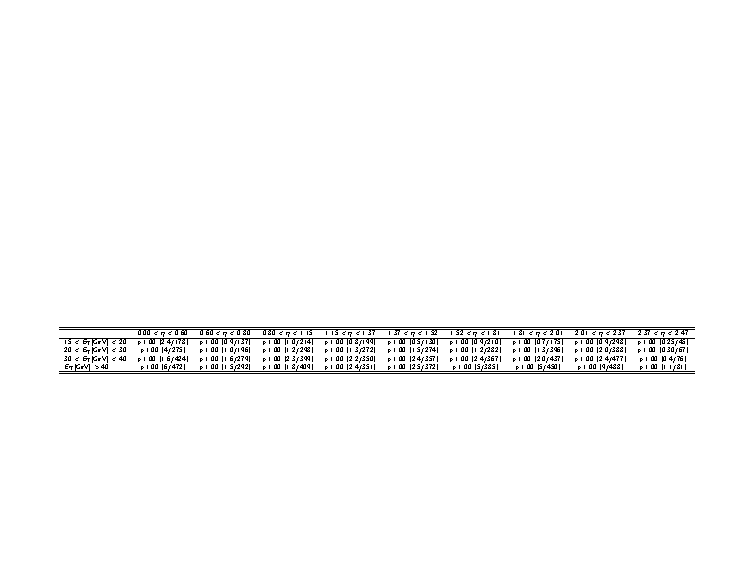
\includegraphics[width=\textwidth]{appendices/figures/gof/eratio_chi2_table.pdf}
\end{subtable} \\
\begin{subtable}{\textwidth}
\caption{\rhad{}\label{tab:gof_chi2_p_values_rhad}}
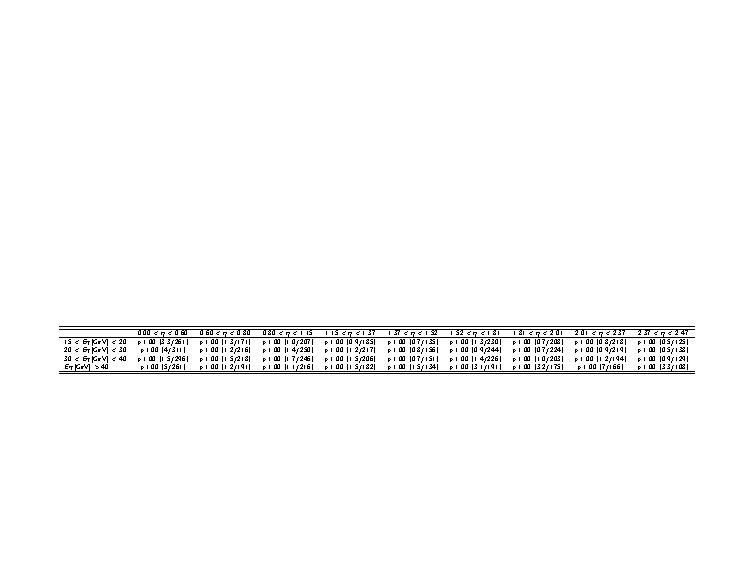
\includegraphics[width=\textwidth]{appendices/figures/gof/rhad_chi2_table.pdf}
\end{subtable} \\
\begin{subtable}{\textwidth}
\caption{\weta{}\label{tab:gof_chi2_p_values_weta}}
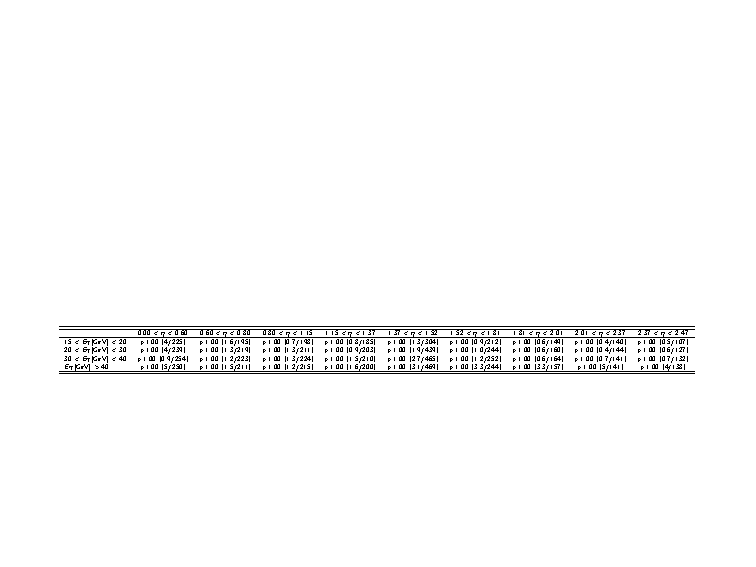
\includegraphics[width=\textwidth]{appendices/figures/gof/weta2_chi2_table.pdf}
\end{subtable} \\
\begin{subtable}{\textwidth}
\caption{\fI{}\label{tab:gof_chi2_p_values_f1}}
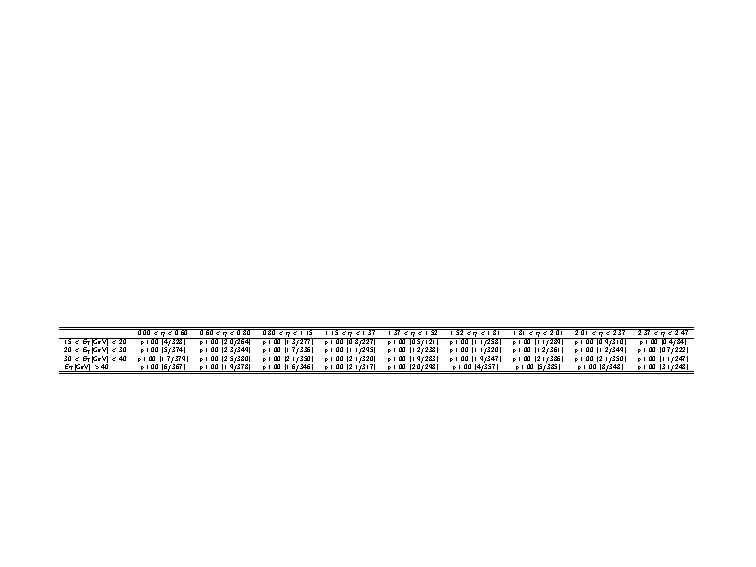
\includegraphics[width=\textwidth]{appendices/figures/gof/f1_chi2_table.pdf}
\end{subtable} \\
\begin{subtable}{\textwidth}
\caption{\fIII{}\label{tab:gof_chi2_p_values_f3}}
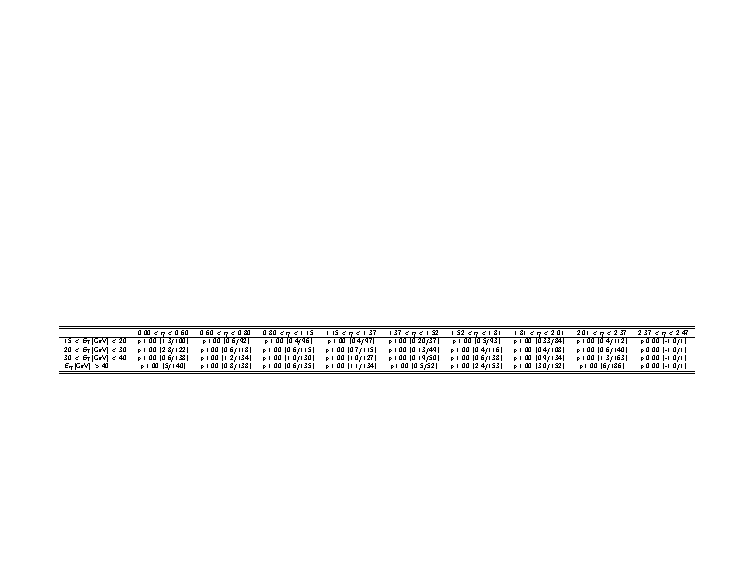
\includegraphics[width=\textwidth]{appendices/figures/gof/f3_chi2_table.pdf}
\end{subtable} \\
\begin{subtable}{\textwidth}
\caption{\TRTPID{}\label{tab:gof_chi2_p_values_trt}}
\includegraphics[width=\textwidth]{appendices/figures/gof/TRT_PID_chi2_table.pdf}
\end{subtable} \\
\begin{subtable}{\textwidth}
\caption{\deltaeta{}\label{tab:gof_chi2_p_values_eta}}
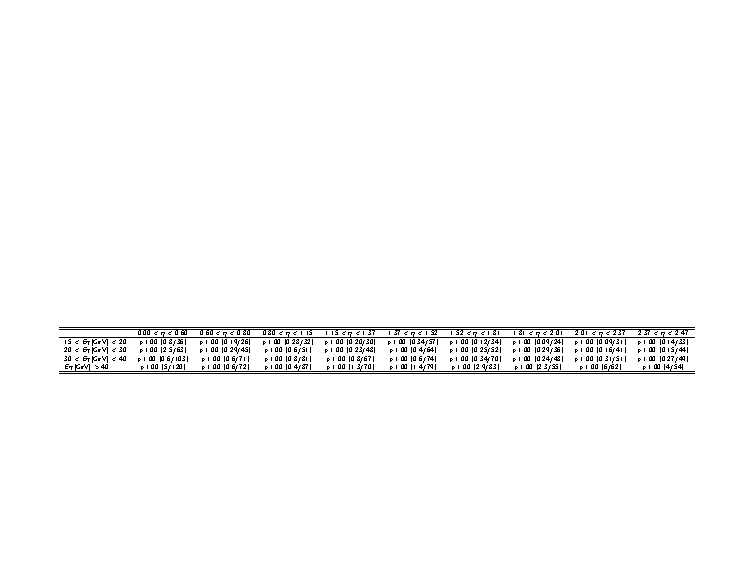
\includegraphics[width=\textwidth]{appendices/figures/gof/deltaeta_chi2_table.pdf}
\end{subtable} \\
\end{table}%
\begin{table}[t]\ContinuedFloat\addtocounter{table}{-1}%
\begin{subtable}{\textwidth}
\caption{\deltaphires{}\label{tab:gof_chi2_p_values_deltaphi}}
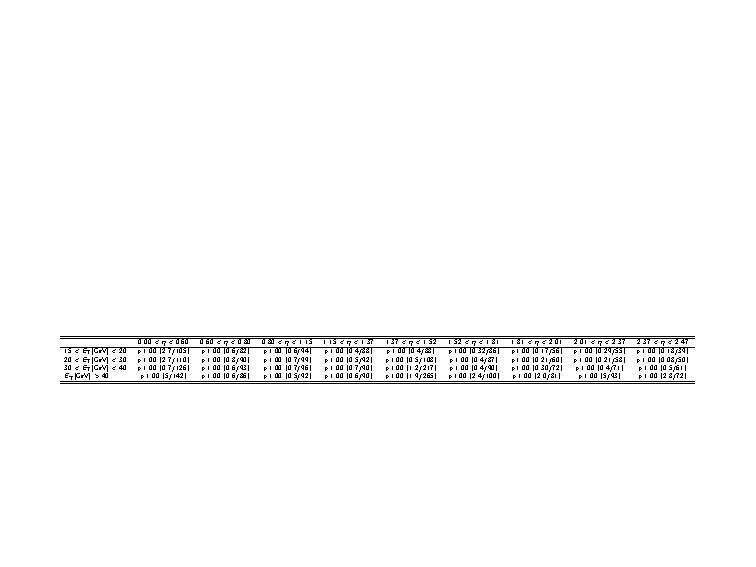
\includegraphics[width=\textwidth]{appendices/figures/gof/deltaphi_chi2_table}
\end{subtable} \\
\begin{subtable}{\textwidth}
\caption{\deltapoverp{}\label{tab:gof_chi2_p_values_poverp}}
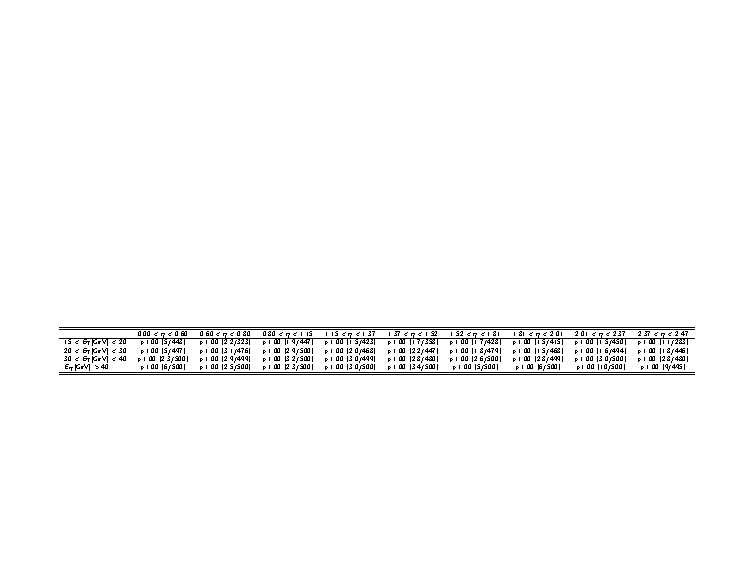
\includegraphics[width=\textwidth]{appendices/figures/gof/deltapoverp_chi2_table.pdf}
\end{subtable} \\
\begin{subtable}{\textwidth}
\caption{\trackdO{}\label{tab:gof_chi2_p_values_d0}}
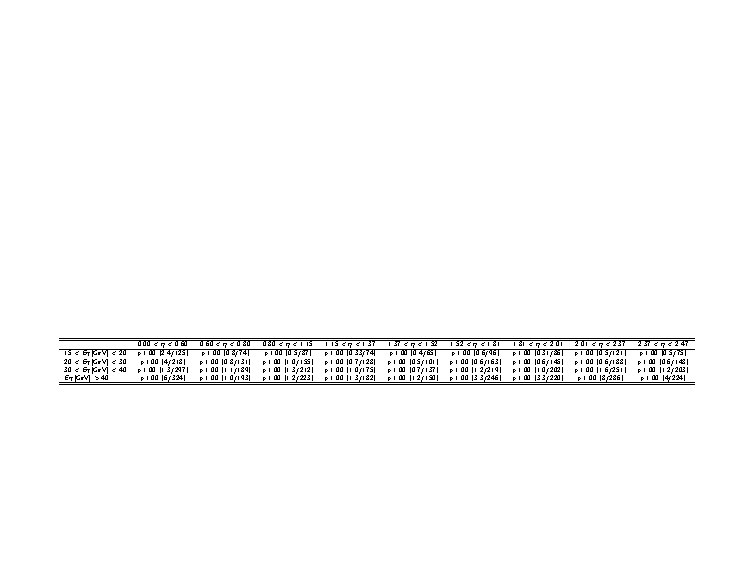
\includegraphics[width=\textwidth]{appendices/figures/gof/d0_chi2_table.pdf}
\end{subtable} \\
\begin{subtable}{\textwidth}
\caption{\dOSignificance{}\label{tab:gof_chi2_p_values_d0sig}}
\includegraphics[width=\textwidth]{appendices/figures/gof/d0sig_chi2_table}
\end{subtable} \\
\end{table}

\begin{table}[b]
\centering
\caption{\label{tab:gof_ks_p_values}Goodness-of-fit test p-value and cumulated
  $\chi^2/\text{ndf}$ for all variables and $\et{}\times\eta{}$
  regions employed to derive the offline likelihood pdfs.}
\begin{subtable}{\textwidth}
\caption{\reta{}\label{tab:gof_ks_p_values_reta}}
\includegraphics[width=\textwidth]{appendices/figures/gof/reta_ks_table.pdf}
\end{subtable} \\
\begin{subtable}{\textwidth}
\caption{\rphi{}\label{tab:gof_ks_p_values_rphi}}
\includegraphics[width=\textwidth]{appendices/figures/gof/rphi_ks_table.pdf}
\end{subtable} \\
\begin{subtable}{\textwidth}
\caption{\eratio{}\label{tab:gof_ks_p_values_eratio}}
\includegraphics[width=\textwidth]{appendices/figures/gof/eratio_ks_table.pdf}
\end{subtable} \\
\begin{subtable}{\textwidth}
\caption{\rhad{}\label{tab:gof_ks_p_values_rhad}}
\includegraphics[width=\textwidth]{appendices/figures/gof/rhad_ks_table.pdf}
\end{subtable} \\
\begin{subtable}{\textwidth}
\caption{\weta{}\label{tab:gof_ks_p_values_weta}}
\includegraphics[width=\textwidth]{appendices/figures/gof/weta2_ks_table.pdf}
\end{subtable} \\
\end{table}%
\begin{table}[p]\ContinuedFloat\addtocounter{table}{-1}%
\begin{subtable}{\textwidth}
\caption{\fI{}\label{tab:gof_ks_p_values_f1}}
\includegraphics[width=\textwidth]{appendices/figures/gof/f1_ks_table.pdf}
\end{subtable} \\
\begin{subtable}{\textwidth}
\caption{\fIII{}\label{tab:gof_ks_p_values_f3}}
\includegraphics[width=\textwidth]{appendices/figures/gof/f3_ks_table.pdf}
\end{subtable} \\
\begin{subtable}{\textwidth}
\caption{\TRTPID{}\label{tab:gof_ks_p_values_trt}}
\includegraphics[width=\textwidth]{appendices/figures/gof/TRT_PID_ks_table.pdf}
\end{subtable} \\
\begin{subtable}{\textwidth}
\caption{\deltaeta{}\label{tab:gof_ks_p_values_eta}}
\includegraphics[width=\textwidth]{appendices/figures/gof/deltaeta_ks_table.pdf}
\end{subtable} \\
\begin{subtable}{\textwidth}
\caption{\deltaphires{}\label{tab:gof_ks_p_values_deltaphi}}
\includegraphics[width=\textwidth]{appendices/figures/gof/deltaphi_ks_table}
\end{subtable} \\
\begin{subtable}{\textwidth}
\caption{\deltapoverp{}\label{tab:gof_ks_p_values_poverp}}
\includegraphics[width=\textwidth]{appendices/figures/gof/deltapoverp_ks_table.pdf}
\end{subtable} \\
\begin{subtable}{\textwidth}
\caption{\trackdO{}\label{tab:gof_ks_p_values_d0}}
\includegraphics[width=\textwidth]{appendices/figures/gof/d0_ks_table.pdf}
\end{subtable} \\
\begin{subtable}{\textwidth}
\caption{\dOSignificance{}\label{tab:gof_ks_p_values_d0sig}}
\includegraphics[width=\textwidth]{appendices/figures/gof/d0sig_ks_table}
\end{subtable} \\
\end{table}
\FloatBarrier

\begin{figure}[b]
\begin{center}
\begin{subfigure}[c]{.48\textwidth}
\centering
\includegraphics[width=\textwidth]{appendices/figures/noAdjustment/marginal_nosplit/e28_MergedRuns/base_new/el_trackd0pvunbiased_et40eta0_00_sigma_base_new.pdf}
\caption{}%
\label{fig:gof_d0}
\end{subfigure}
\hfill
\begin{subfigure}[c]{.48\textwidth}
\centering
\includegraphics[width=\textwidth]{appendices/figures/noAdjustment/marginal_nosplit/e28_MergedRuns/base_new/el_d0significance_et40eta0_00_sigma_base_new.pdf}
\caption{}%
\label{fig:gof_d0sig}
\end{subfigure} \\
\begin{subfigure}[c]{.48\textwidth}
\centering
\includegraphics[width=\textwidth]{appendices/figures/noAdjustment/marginal_nosplit/e28_MergedRuns/base_new/el_DeltaPoverP_et40eta0_00_sigma_base_new.pdf}
\caption{}%
\label{fig:gof_poverp}
\end{subfigure}
\hfill
\begin{subfigure}[c]{.48\textwidth}
\centering
\includegraphics[width=\textwidth]{appendices/figures/noAdjustment/marginal_nosplit/e28_MergedRuns/base_new/el_TRT_PID_et40eta0_00_sigma_base_new.pdf}
\caption{}%
\label{fig:gof_TRT_PID}
\end{subfigure} \\
\end{center}
\end{figure}%
\begin{figure}[t]\ContinuedFloat\addtocounter{figure}{-1}
\begin{center}
\begin{subfigure}[c]{.48\textwidth}
\centering
\includegraphics[width=\textwidth]{appendices/figures/noAdjustment/marginal_nosplit/e28_MergedRuns/base_new/el_deltaeta1_et40eta0_00_sigma_base_new.pdf}
\caption{}%
\label{fig:gof_deltaeta1}
\end{subfigure}
\begin{subfigure}[c]{.48\textwidth}
\centering
\includegraphics[width=\textwidth]{appendices/figures/noAdjustment/marginal_nosplit/e28_MergedRuns/base_new/el_deltaphiRescaled_et40eta0_00_sigma_base_new.pdf}
\caption{}%
\label{fig:gof_deltaphi}
\end{subfigure}
\caption{%
Histogram profiles for the ID and calo-ID combined variables employed in
the offline likelihood in the $\et>\SI{40}{\GeV}$ and $0.00<\abseta{}<0.80$
region using the trigger without \rnn{} (blue area) and with \rnn{}
(black line).
}%
\label{fig:gof_track}
\end{center}
\end{figure}

\FloatBarrier
\subsubsection{Pseudo-Experiments}%
\label{top:pseudo_extra}

Figure~\ref{fig:pseudo_counts} shows the counts and percentage difference of
\tnp{} pairs for the pseudo-experiment approach. Figure~\ref{fig:pseudo_track}
shows the ID and calo-ID combined variables employed in the offline likelihood
algorithm.

\begin{figure}[b]
\begin{center}
\begin{subfigure}[c]{.48\textwidth}
\centering
\includegraphics[width=\textwidth]{appendices/figures/noAdjustment/marginal_mutually_exclusive/e28_MergedRuns_mutuallyExclusive/bonly_nonly/probe_count0_bonly_nonly.pdf}
\caption{}%
\label{fig:pseudo_counts_without_ringer}
\end{subfigure}
\begin{subfigure}[c]{.48\textwidth}
\centering
\includegraphics[width=\textwidth]{appendices/figures/noAdjustment/marginal_mutually_exclusive/e28_MergedRuns_mutuallyExclusive/bonly_nonly/probe_count1_bonly_nonly.pdf}
\caption{}%
\label{fig:pseudo_counts_with_ringer}
\end{subfigure} \\
\hspace*{\fill}
\begin{subfigure}[c]{.48\textwidth}
\centering
\caption{}%
\includegraphics[width=\textwidth]{appendices/figures/noAdjustment/marginal_mutually_exclusive/e28_MergedRuns_mutuallyExclusive/bonly_nonly/delta_perc_bonly_nonly.pdf}
\label{fig:pseudo_delta_perc}
\end{subfigure}
\hspace*{\fill} \\
\caption{%
  Probe counts per phase space region for the trigger with (a) and without (b)
  \rnn{}. The difference percentage between the two triggers is shown at the
  bottom (c).
}%
\label{fig:pseudo_counts}
\end{center}
\end{figure}

\begin{figure}[htb]
\begin{center}
\begin{subfigure}[c]{.48\textwidth}
\centering
\includegraphics[width=\textwidth]{appendices/figures/noAdjustment/marginal_mutually_exclusive/e28_MergedRuns_mutuallyExclusive/bonly_nonly/el_trackd0pvunbiased_et40eta0_00_kldivergence_bonly_nonly.pdf}
\caption{}%
\label{fig:pseudo_d0}
\end{subfigure}
\hfill
\begin{subfigure}[c]{.48\textwidth}
\centering
\includegraphics[width=\textwidth]{appendices/figures/noAdjustment/marginal_mutually_exclusive/e28_MergedRuns_mutuallyExclusive/bonly_nonly/el_d0significance_et40eta0_00_kldivergence_bonly_nonly.pdf}
\caption{}%
\label{fig:pseudo_d0significance}
\end{subfigure} \\
\begin{subfigure}[c]{.48\textwidth}
\centering
\includegraphics[width=\textwidth]{appendices/figures/noAdjustment/marginal_mutually_exclusive/e28_MergedRuns_mutuallyExclusive/bonly_nonly/el_DeltaPoverP_et40eta0_00_kldivergence_bonly_nonly.pdf}
\caption{}%
\label{fig:pseudo_poverp}
\end{subfigure}
\hfill
\begin{subfigure}[c]{.48\textwidth}
\centering
\includegraphics[width=\textwidth]{appendices/figures/noAdjustment/marginal_mutually_exclusive/e28_MergedRuns_mutuallyExclusive/bonly_nonly/el_TRT_PID_et40eta0_00_kldivergence_bonly_nonly.pdf}
\caption{}%
\label{fig:pseudo_TRT_PID}
\end{subfigure} \\
\end{center}
\end{figure}%
\begin{figure}[t]\ContinuedFloat
\begin{center}
\begin{subfigure}[c]{.48\textwidth}
\centering
\includegraphics[width=\textwidth]{appendices/figures/noAdjustment/marginal_mutually_exclusive/e28_MergedRuns_mutuallyExclusive/bonly_nonly/el_deltaeta1_et40eta0_00_kldivergence_bonly_nonly.pdf}
\caption{}%
\label{fig:pseudo_deta}
\end{subfigure}
\hfill
\begin{subfigure}[c]{.48\textwidth}
\centering
\includegraphics[width=\textwidth]{appendices/figures/noAdjustment/marginal_mutually_exclusive/e28_MergedRuns_mutuallyExclusive/bonly_nonly/el_deltaphiRescaled_et40eta0_00_kldivergence_bonly_nonly.pdf}
\caption{}%
\label{fig:pseudo_dphi}
\end{subfigure}
\caption{Profiles for the disagreements between
  the trigger with and without \rnn{} for each ID and calo-ID variable employed
in the offline likelihood in the $\et>\SI{40}{\GeV}$ and $0.00<\abseta{}<0.80$
region.}%
\label{fig:pseudo_track}
\end{center}
\end{figure}
